% 
% Sjabloon voor de master ingenieurswetenschappen: computerwetenschappen
%
\documentclass[master=cws]{kulemt}
%%%%%%%%%%%%%%  Wijzig niets boven deze regel  %%%%%%%%%%%%%
% 
% Vul de titel van jouw masterproef hieronder in tussen { en }.
\setup{title={Melodische transformatie en evalutie van muziek},
%
% Vul hieronder namen in, steeds Voornaam Naam.
% Indien meerdere auteurs, assessoren, assistenten, scheidt hun namen
%   met \and .
  author={Elias Moons},
  promotor={Prof.\,dr.\,D. De Schreye},
  assessor={Prof. Onbekend},
  assistant={Ir.\ V. Nys}}
% 
\setup{filingcard,   % Deze regel niet wijzigen
%
% Vul de vertaalde titel van jouw masterproef hieronder in tussen { en }.
  translatedtitle={Melodische transformatie en evalutie van muziek},
%
% UDC nummer is richtingafhankelijk. 
% Zie http://www.udcc.org/udcsummary/php/index.php
% voor het UDC nummer.
% Dit voorbeeld (519.6) verwijst naar 'Computational mathematics'
  udc=004.9,
%
% Hieronder, tussen { en } een korte samenvatting toevoegen.
% Lege regels en het commando \par zijn niet toegelaten.
% Wees voorzichtig met speciale TeX-tekens #$%&^_~{}\ !!
  shortabstract={%
    Hier komt een heel bondig abstract van hooguit 500
    woorden. \LaTeX\ commando's mogen hier gebruikt worden.
    Voorbeelden van letters met accenten zijn 
    ``{\'e}{\"\i}{\c{c}}{\`a}{\^o}''.
   (Gebruik {\"\i} in plaats van {\"i}, om geen 3 puntjes te hebben.)
   }}
% Verwijder de "%" op de volgende lijn als je de kaft wil afdrukken
%\setup{coverpageonly}
% Verwijder de "%" op de volgende lijn als je enkel de eerste pagina's wil
% afdrukken en de rest bv. via Word aanmaken.
%\setup{frontpagesonly}

% Kies de fonts voor de gewone tekst, bv. Latin Modern
\setup{font=lm}

% Hier kun je dan nog andere pakketten laden of eigen definities voorzien

% Tenslotte wordt hyperref gebruikt voor pdf bestanden.
% Dit mag verwijderd worden voor de af te drukken versie.
\usepackage[pdfusetitle,colorlinks,plainpages=false]{hyperref}

%%%%%%%
% Om wat tekst te genereren wordt hier het lipsum pakket gebruikt.
% Bij een echte masterproef heb je dit natuurlijk nooit nodig!
\IfFileExists{lipsum.sty}%
 {\usepackage{lipsum}\setlipsumdefault{11-13}}%
 {\newcommand{\lipsum}[1][11-13]{\par Hier komt wat tekst: lipsum ##1.\par}}
%%%%%%%

%Eigen toegevoegde packages
\usepackage{pdfpages}
\usepackage{amsmath} %tijdssignatuur muziekstuk
\usepackage{xr} %cross referencing tussen verschillende tex files
\externaldocument{1_Muzikale_Achtergrond/muzikale_achtergrond}
\externaldocument{2_Objectieve_Beoordeling/objectieve_beoordeling}
\externaldocument{3_Melodische_Transformatie/melodische_transformatie}
\externaldocument{4_Efficient_Toepassen_Transformatie/efficient_toepassen_transformatie}
\externaldocument{5_Experimenten_Resultaten/experimenten_resultaten}
\externaldocument{6_Besluit/besluit}
\externaldocument{Appendix_0_Broncode/broncode}
\usepackage{listings}
\lstset{breaklines}
\usepackage{tikz}

\begin{document}

\begin{preface}
  TODO: iedereen bedanken...
\end{preface}

\tableofcontents*

\begin{abstract}
  Deze masterproef beschrijft methodes om melodielijnen van een muziekstuk melodisch te transformeren to nieuwe melodielijnen. Verder wordt er ook aandacht besteed aan een referentiekader waarin deze transformaties ge\"evalueerd kunnen worden. Tot slot wordt er ook nog gekeken naar wanneer bepaalde transformaties nuttig kunnen zijn om de consonantie van een muziekstuk te verhogen. Om dit te verwezenlijken is een algoritme beschreven dat gebaseerd is op de principes van \textit{dynamic programming}. Dit algoritme zal, gegeven een aantal mogelijke transformaties en een melodielijn, de best mogelijke getransformeerde melodielijn teruggeven, dit volgens het gedefini\"eerde referentiemodel.
\end{abstract}

% Een lijst van figuren en tabellen is optioneel
%\listoffigures
%\listoftables
% Bij een beperkt aantal figuren en tabellen gebruik je liever het volgende:
\listoffiguresandtables
% De lijst van symbolen is eveneens optioneel.
% Deze lijst moet wel manueel aangemaakt worden, bv. als volgt:
\chapter{Lijst van afkortingen en symbolen}
\section*{Afkortingen}
\begin{flushleft}
  \renewcommand{\arraystretch}{1.1}
  \begin{tabularx}{\textwidth}{@{}p{12mm}X@{}}
    LoG   & Laplacian-of-Gaussian \\
    MSE   & Mean Square error \\
    PSNR  & Peak Signal-to-Noise ratio \\
  \end{tabularx}
\end{flushleft}
\section*{Symbolen}
\begin{flushleft}
  \renewcommand{\arraystretch}{1.1}
  \begin{tabularx}{\textwidth}{@{}p{12mm}X@{}}
    42    & ``The Answer to the Ultimate Question of Life, the Universe,
            and Everything'' volgens de \cite{h2g2} \\
    $c$   & Lichtsnelheid \\
    $E$   & Energie \\
    $m$   & Massa \\
    $\pi$ & Het getal pi \\
  \end{tabularx}
\end{flushleft}

% Nu begint de eigenlijke tekst
\mainmatter

\chapter{Inleiding}
\label{hoofdstuk:I}
%In dit hoofdstuk wordt het werk ingeleid. Het doel wordt gedefinieerd en er
%wordt uitgelegd wat de te volgen weg is (beter bekend als de rode draad).

%Als je niet goed weet wat een masterproef is, kan je altijd
%Wikipedia\cite{wiki} eens nakijken.

\section{Probleemstelling}
Een van de meest voorkomende problemen voor muzikanten is de zogenaamde \textit{writer's block}. Dit fenomeen waarbij je als muzikant merkt dat je de hele tijd op hetzelfde melodietje uitkomt en maar niet met iets nieuw kan komen kan zeer frustrerend zijn. Daarom zou het handig zijn als er een tool zou bestaan die je als het ware de inspiratie kan geven die je nodig hebt om deze \textit{writer's block} te doorbreken. Een mogelijke oplossing voor dit probleem wordt in deze thesis onderzocht. Hier gaat het dan om het transformeren van reeds gekende melodie\"en tot nieuwe melodie\"en.

\section{Vergelijking met voorgaand onderzoek}
Onderzoek naar het bekomen van nieuwe melodie\"en waarbij gebruik gemaakt wordt van een computer is niet nieuw \cite{thesis:thomas} \cite{book:musicAndProbability}. Al gedurende tientallen jaren is er veel werk geleverd op het vlak van muziekgeneratie, waarbij het de bedoeling is om een muziekstuk te genereren waarbij vertrokken wordt van een lege partituur \cite{book:musicGeeksNerds}. Dit wordt gedaan rekening houdend met de regels uit de muziektheorie en vaak probeert men er ook een vorm van repetitiviteit en herkenning in te brengen zoals vaak ook het geval is in hedendaagse muziek. 

Een groot probleem dat echter altijd terugkwam was dat het heel moeilijk was om een goede verhouding te vinden tussen twee heel belangrijke eigenschappen van de muziek, namelijk verwachting en verrassing van de luisteraar \cite{book:musimathics}. Een luisteraar heeft namelijk een bepaald verwachtingspatroon voor het onmiddellijke vervolg van een melodie. Dit verwachtingspatroon strookt vaak met de regels van de muziektheorie. Wanneer deze regels dan weer te nauwgezet gevolgd worden, wordt het muziekstuk als saai ervaren, er is dus nood aan een zekere verrassing in de melodie. Te veel onverwachte wendingen worden dan weer als frustrerend gezien, kortom, het is van cruciaal belang om een goed evenwicht te vinden tussen deze twee waarden. Dit blijkt zeer moeilijk te verwezenlijken vanuit het standpunt van muziekgeneratie.\\

\section{Doelstelling}
In deze thesis wordt een onderzoek gevoerd naar de generatie van nieuwe melodie\"en vertrekkende van originele melodie\"en. Deze originele melodie\"en worden bij aanname verondersteld te voldoen aan de eisen van verrassing en verwachting. In deze thesis worden specifiek melodische transformaties onderzocht. Deze transformaties zullen gebaseerd zijn op wiskundige reeksen. Hierbij gaat men voor elke noot in de oorspronkelijke melodie de toonhoogte aanpassen volgens een bepaald patroon. Als voorbeeld om het concept te verduidelijken kan figuur \ref{figuur:fibo} dienen. In deze figuur wordt met behulp van de rij van Fibonacci een originele melodie getransformeerd tot een nieuwe. 

Er wordt getracht zo een transformatie te zoeken zodat de nieuw bekomen melodie nog steeds consonant is (nog steeds goed klinkt). Er zal ook onderzocht worden onder welke omstandigheden een transformatie al dan niet een consonante melodie oplevert. Om te bepalen of een nieuwe melodie goed klinkt is er ook nood aan een objectieve beoordeling van melodie\"en. Er wordt dus ook aandacht besteed aan het opstellen van een model dat hiervoor kan dienen. Een model dat zo goed mogelijk kan beoordelen of een gegeven melodie al dan niet, en in welke mate, consonant is. Het voordeel van het werken met transformaties in plaats van met generatie is dat men op deze manier nog een deel van de eigenheid van het originele werk kan behouden en het bekomen werk hierdoor ook minder artificieel zal overkomen bij de luisteraar.

\begin{figure}[!ht]
  \centering
  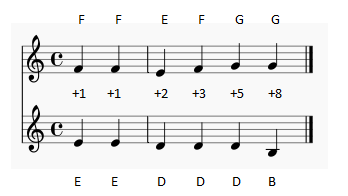
\includegraphics[width=0.5\textwidth]{0_Inleiding/fibo}
  \caption{Melodische transformatie m.b.v. rij van Fibonacci: Noten op de bovenste notenbalk liggen respectievelijk 1,1,2,3,5,8 halve tonen hoger dan op de onderste notenbalk.}
  \label{figuur:fibo}
\end{figure}

\section{Assumpties en beperkingen}
Op een onderdeel van hoofdstuk \ref{hoofdstuk:OBM} na, behandelt deze masterproef enkel muziek met precies \'e\'en melodielijn. Meerstemmige muziek waarbij meerdere noten tegelijkertijd gespeeld kunnen worden, wordt in deze thesis dus niet behandeld. Verder worden alle testen uitgevoerd op een corpus (Essencorpus \cite{url:essen}) bestaande uit muziekstukken van het folk genre.

Tot slot zal ook telkens wanneer een transformatie uitgevoerd is, er vanuit gegaan worden dat het originele muziekstuk telkens voldoet aan de algemene voorwaarden waaraan een muziekstuk moet voldoen. In dat geval kan de score van dit muziekstuk in het voorgestelde model telkens ook als referentie dienen voor de getransformeerde versie. 

\section{Overzicht van de tekst}
In het eerstvolgende hoofdstuk, hoofdstuk \ref{hoofdstuk:MA} wordt een korte inleiding gegeven tot de muziektheorie. Hierin worden enkel deze elementen behandeld die relevant zijn voor de rest van deze thesis. Vervolgens zal er besproken worden hoe de kwaliteit van een muziekstuk objectief beoordeeld kan worden, dit zal gebeuren in hoofdstuk \ref{hoofdstuk:OBM}. In hoofdstuk \ref{hoofdstuk:MT} worden verschillende melodische transformaties toegelicht en met elkaar vergeleken. Vervolgens zal hoofdstuk \ref{hoofdstuk:ETT} twee algoritmes beschrijven. Deze algoritmes kunnen gebruikt worden om gegeven een aantal toegestane transformaties en een oorspronkelijke melodielijn, de meest waarschijnlijke getransformeerde melodielijn terug te geven. Hierna zullen een aantal experimenten, alsook hun resultaten besproken worden in hoofdstuk \ref{hoofdstuk:ER}. Tot slot wordt er in hoofdstuk \ref{hoofdstuk:B} nog teruggekeken op het geleverde onderzoek in een samenvattend besluit. Er wordt ook nog beschreven welk verder onderzoek zeker nog interessant zou kunnen zijn over dit onderwerp. 

%%% Local Variables: 
%%% mode: latex
%%% TeX-master: "masterproef"
%%% End: 

\newcommand{\signatuur}[2]{\ensuremath{%
  \vcenter{\offinterlineskip
    \halign{\hfil##\hfil\cr
            $\scriptstyle#1$\cr
            \noalign{\vskip1pt}
            $\scriptstyle#2$\cr}
  }}%
}

\chapter{Muzikale Achtergrond}
\label{hoofdstuk:MA}

Aangezien deze thesis zal handelen over melodische transformaties wordt hieronder in het kort info gegeven over elementaire begrippen rond ritme en melodie van een muziekstuk en hoe deze voorgesteld kunnen worden. Voor lezers met een voorkennis in de muziekwereld zal dit onderdeel waarschijnlijk redundant zijn en kan er bijgevolg ook meteen overgegaan worden naar het volgende hoofdstuk. 

\section{Ritme}
In deze masterproef worden enkel melodische transformaties behandeld, waarbij het ritme ongewijzigd blijft. Toch is het zeker nuttig om ook een zekere voorkennis te hebben van de betekenis van ritme in een muziekstuk. Melodie en ritme van een muziekstuk gaan namelijk hand in hand. Een basiskennis van ritmische begrippen zal dus zeker ook nuttig zijn voor het begrijpen van bepaalde melodische fenomenen.  

\subsection{Tijdssignaturen}
De tijdssignatuur geeft de ritmische structuur weer van het muziekstuk. Deze tijddssignatuur wordt weergegeven aan het begin van de notenbalk en ziet er uit als een breuk zonder streepje. Een voorbeeld hiervan is de vaak gebruikte \signatuur{3}{4} (of 'drie vierden'). In deze voorstelling staat het onderste getal voor welke nootlengte overeen komt met een tel. Het bovenste getal geeft weer hoeveel tellen in een maat voorkomen. In het voorbeeld van de signatuur \signatuur{3}{4} komt dit over met 4 tellen van lengte $\frac{1}{4}$. Voor de specifieke signatuur \signatuur{4}{4} (of 'vier vierden') heeft men nog een andere notatie, namelijk de letter C. Deze letter komt het woord \textit{common time}, aangezien deze signatuur zo typisch en veelvoorkomend is in moderne Westerse muziek. Figuur \ref{figuur:tijdssignatuur} geeft het gebruik van deze notatie weer. De figuur illustreert ook de 4 verschillende tellen van deze maatsoort.

\begin{figure}[!ht]
  \centering
  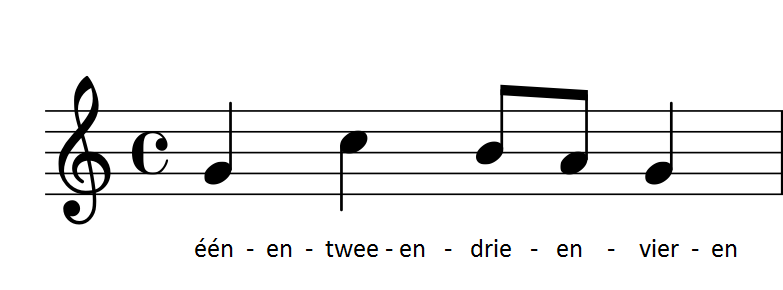
\includegraphics[width=0.5\textwidth]{1_Muzikale_Achtergrond/tijdssignatuur}
  \caption{Maat met voortekening van \textit{common time} tijdssignatuur.}
  \label{figuur:tijdssignatuur}
\end{figure}

\subsection{Tempo}
Een volgend belangrijk onderdeel dat het ritme van een muziekstuk bepaalt is het tempo. Het tempo van een stuk bepaalt namelijk de duur van de verschillende noten in het muziekstuk. Het temp wordt meestal uitgedrukt in aantal tellen per minuut. De lengte van een tel zelf wordt dan weer bepaald door de tijdssignatuur. Zo betekent bijvoorbeeld een tempo van 60 tellen voor een muziekstuk met signatuur \signatuur{3}{4} dat elke tel, ofwel elke kwartnoot, precies \'e\'en seconde duurt. 

\subsection{Nootlengtes}
De nootlengte is het laatste element dat de absolute duur van een noot zal bepalen. De nootlengte geeft de relatieve lengte van een noot weer ten opzichte van het tempo en de tijdssignatuur. De nootlengte wordt uitgedrukt door een breuk. Deze breuk heeft als relatieve lengte zijn verhouding tot de lengte van een tel. Zo zal een $\frac{1}{4}$-noot in \signatuur{3}{4} \'e\'en tel duren, en zal een $\frac{1}{8}$-noot in \signatuur{3}{4} twee tellen duren.\\
Een note van hele lengte wordt aangeduid met een hol bolletje. Een noot van halve lengte wordt aangeduid met een half bolletje met een streep aan de rechterkant. Een $\frac{1}{4}$-noot wordt aangeduid zoals een halve noot maar dan met een vol bolletje. Een $\frac{1}{8}$-noot wordt voorgesteld door een vierde noot met een streepje vanboven. Vanaf een $\frac{1}{16}$-noot wordt er dan een streepje vanboven bijgezet telkens de nootlengte gehalveerd wordt. Deze notatie wordt ge\"illustreerd in figuur \ref{figuur:toonlengtes}. Door het gebruik van verbindingstekens(waarbij de nieuwe nootlengte de som is van de lengtes van de twee noten die verbonden zijn) kan men dan eender welke nootlengte bekomen die men maar wenst. 

\begin{figure}[!ht]
  \centering
  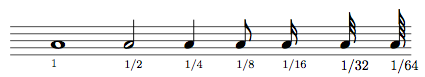
\includegraphics[width=0.5\textwidth]{1_Muzikale_Achtergrond/nootlengtes}
  \caption{Illustratie van een aantal veelvoorkomende nootlengtes.}
  \label{figuur:nootlengtes}
\end{figure}

\section{Melodie}
Naast ritme is het andere fundamentele bestanddeel van een muziekstuk de melodie. Waar het ritme de structuur van een muziekstuk weergeeft, is de melodie het voornaamste bestanddeel van de muziek dat een gevoel meegeeft aan het stuk. De melodie geeft een toonhoogte of freqentie mee aan elke noot. Aangezien deze thesis handelt over melodische transformaties is het van belang te weten wat het begrip `melodie' precies inhoudt. Het is namelijk dat gedeetle van een muziekstuk waarop een transformatie zal toegepast worden. Het ritme van een muziekstuk wordt in deze thesis onveranderd gelaten.

\subsection{Toonhoogte}
Toonhoogte kan in het algemeen op twee manieren voorgesteld worden. Een eerste manier is fysische waarbij elke toon met een bepaalde frequentie overeenkomt, een andere manier is meer muziek-theoretisch, waarbij de toonhoogte als discreet beschouwd wordt. In deze masterproef zal met de laatste voorstellingswijze gewerkt worden. Dit omdat we noten willen transformeren naar nieuwe noten en niet frequenties naar nieuwe frequenties (die dan niet overeen komen met een noot en bijgevolg zeer waarschijnlijk niet goed gaan klinken in het geheel). Deze toonhoogte wordt dan voorgesteld door een naam. Er zijn twee naamgevingen die vaak gebruikt worden. Eerst is er de naamgeving waarbij de letters A t.e.m. G gebruikt worden. De andere naamgeving maakt gebruik van de woorden do -- re -- mi -- fa -- sol -- la -- si, de relatie tussen deze 2 naamgevingen wordt weergegeven in tabel \ref{tabel:toonhoogte}. Noten kunnen uiteraard ook op een notenbalk weergegeven worden, zie figuur \ref{figuur:toonladder} voor een visuele weergave. Hoe hoger de noot op de notenbalk, hoe hoger haar frequentie.

\begin{table}
  \centering
  \begin{tabular}{ c c c c c c c }
    A & B & C & D & E & F & G \\
    \hline
    \hline
    la & si & do & re & mi & fa & sol \\
  \end{tabular}
  \caption{Opsomming van de toonhoogtes in 2 verschillende benamingen.}
  \label{tabel:toonhoogte}
\end{table}

\begin{figure}[!ht]
  \centering
  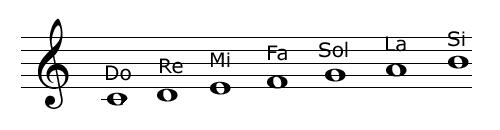
\includegraphics[width=0.5\textwidth]{1_Muzikale_Achtergrond/toonladder}
  \caption{Noten do t.e.m. si op een notenbalk.}
  \label{figuur:toonladder}
\end{figure}

\subsection{Octaaf en onderverdeling in toonhoogtes}
Een eenvoudige definitie van een octaaf is het interval tussen een gegeven toonhoogte en de toonhoogte met het dubbele van de frequentie van de eerste. Deze noten worden als zeer gelijkaardig ervaren en krijgen daarom dezefde benaming (bijvoorbeeld beide een A). Hierdoor gaat men vaak in muzieknotatie wanneer men een bepaalde noot benoemt, ook aangeven tot welk octaaf de noot behoort (want een bepaalde noot komt met meerdere toonhoogtes overeen). Dit doet men door in subscript de index van het octaaf weer te geven, een A (of la) in het vierde octaaf wordt dan weergegeven door $A_{4}$.\\
Een octaaf wordt opgedeeld in 12 toonhoogtes. De afstand tussen elk paar van 2 opeenvolgende toonhoogtes wordt een halve toon genoemd. Hiervan zijn er slechts 7 tonen die ook deel uitmaken van de toonladder. De andere 5 noten worden voorgesteld op de notenbalk relatief ten opzichte van een van de nabijgelegen tonen die slechts een halve toon hier vanaf ligt door het gebruik van een kruis ($\sharp$) of een mol($\flat$). Een kruis dient om aan te duiden dat de noot die bedoeld wordt een halve toon hoger is dan de noot die ervoor staat. Een mol gebruikt men om aan te duiden dat de noot die bedoeld wordt een halve toon lager is dan de noot die net voor het molteken staat.

\subsection{Toonladders en toonaarden}
Zoals reeds vermeld werd in het vorige deel, bestaat een octaaf uit 12 tonen waarvan er slechts 7 tot de eigenlijke toonladder behoren. De noten binnen een toonladder worden bepaald door de intervallen tussen de noten. In het algemeen zijn er twee grote onderverdelingen om een toonladder te construeren. Een eerste resultaat wordt de ``grote toonladder'' genoemd. deze wordt bepaald door de opeenvolging van stappen 1-1-$\frac{1}{2}$-1-1-1-$\frac{1}{2}$. Het meeste elementaire voorbeeld van een toonladder die hieraan voldoet is de toonladder van ``Do-Groot'' waarbij volgende noten voldoen aan de opgegeven intervalafstanden: ``do - re - mi - fa - sol - la - si - do'', zoals weergegeven in figuur \ref{figuur:do_groot}. Een tweede mogelijkheid is de zogenaamde ``kleine toonladder''. In deze toonladder komen de intervalafstanden overeen met 1-$\frac{1}{2}$-1-1-$\frac{1}{2}$-1-1. Een concreet voorbeeld hiervan is de toonladder van ``La-Klein'' waarbij deze noten voldoen aan de voorwaarden: ``la - si - do - re - mi - fa - sol - la'', deze wordt ook weergegeven in figuur \ref{figuur:la_klein}. Deze toonladderis de kleine versie van de toonladder van Do groot, aangezien ze dezelfde noten gebruikt, de toonladder is als het ware een verschuiving van die van Do groot. Het verschil tussen beide toonladders is dus de functie van elke noot in de bijhorende toonaarden. En iets wiskundiger verwoord is er ook een verschil van frequentie waarin bepaalde noten voorkomen in muziekstukken horende bij een kleine of grote toonladder \cite{book:musicAndProbability}. Van de kleine toonladders zijn ook nog een harmonische en melodische versie, die nog andere afstanden gebruik, maar aangezien deze niet zo vaak gebruikt worden, zou het te ver leiden deze ook te bespreken.\\
Het feit of een toonladder groot of klein is gaat vaak ook de sfeer bepalen van het muziekstukje. Zo zal een muziekstuk dat geschreven is in een grote toonladder eerder een vrolijk karakter hebben. Dit terwijl een stukje dat geschreven is in een kleine toonladder eerder een droeviger karakter zal hebben. Maar niet alleen de toonladder zelf, ook de noten in de toonladder hebben hun functie. Zo is bijvoorbeeld de eerste noot van een toonladder een rustpunt waarop het muziekstuk vaak be\"eindigd wordt. De vijfde noot wordt de dominant genoemd en is ook sterk vertegenwoordigd in het muziekstuk. Deze nooit cre\"eert namelijk spanning. Vaak wordt deze spanning dan ook opgelost door een overgang naar de eerste noot, als rustpunt.

\begin{figure}[!ht]
  \centering
  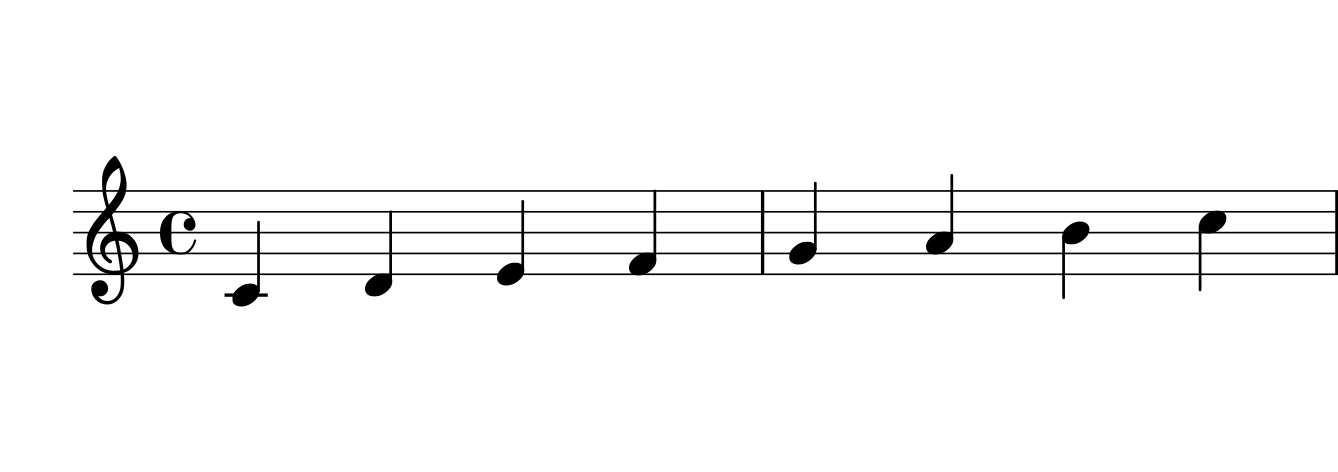
\includegraphics[width=0.5\textwidth]{1_Muzikale_Achtergrond/do_groot}
  \caption{Toonladder van ``Do Groot''}
  \label{figuur:do_groot}
\end{figure}

\begin{figure}[!ht]
  \centering
  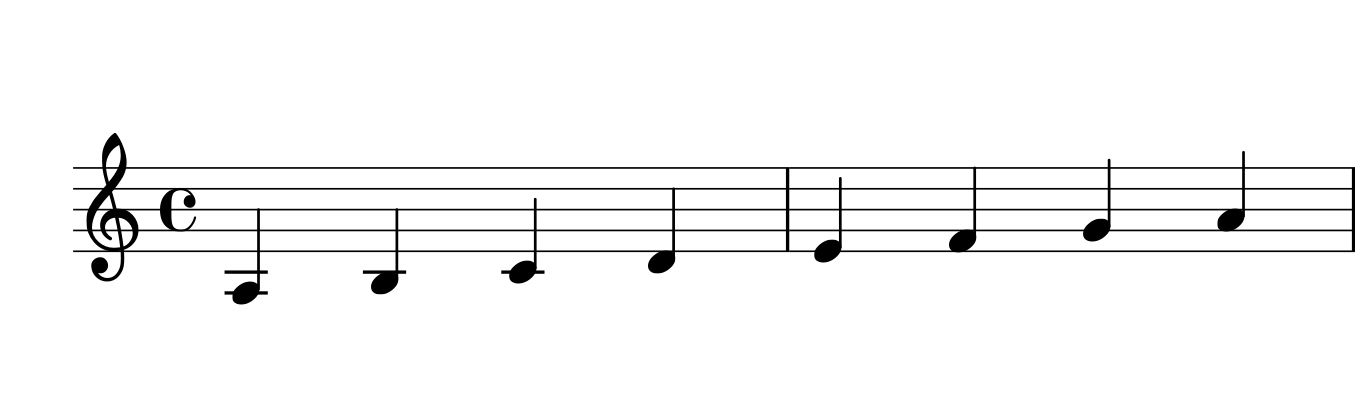
\includegraphics[width=0.5\textwidth]{1_Muzikale_Achtergrond/la_klein}
  \caption{Toonladder van ``La Klein''}
  \label{figuur:la_klein}
\end{figure}

%%% Local Variables: 
%%% mode: latex
%%% TeX-master: "masterproef"
%%% End: 

\chapter{Objectieve Beoordeling Muziekstuk}
\label{hoofdstuk:OBM}
Om melodische transformaties te kunnen beoordelen is er nood aan een framework dat kan voorspellen of een gegeven melodie al dan niet goed klinkt. In dit hoofdstuk worden twee zo een modellen besproken die een bepaalde `consonantiescore' (maat voor het goed klinken van een muziekstuk) gaan toekennen aan een muziekstuk. Allereerst wordt een aanpak besproken die gebruik maakt van een artifici\"eel neuraal netwerk \cite{book:ANN}. Deze methode is speciaal gemaakt voor het beoordelen van polyfone muziek, waarbij er meerdere noten tegelijk klinken. Polyfone muziek wordt in verdere hoofdstukken van deze masterproef niet meer besproken. Het eerste onderdeel van dit hoofdstuk zal bijgevolg dus weinig invloed hebben op het vervolg van de tekst. De methode is echter wel onderzocht geweest en leverde enkele interessante resultaten op waardoor de methode toch even in het kort vermeld wordt. Als tweede methode wordt een zogenaamd `RPK-Model' besproken dat gebaseerd is op een gelijknamig model uit het boek `Music and Probability' \cite{book:musicAndProbability} van David Temperley \cite{url:temperley}. Dit model werkt op muziek met een enkele melodielijn en zal ook het model zijn dat als verificator gebruikt zal worden bij de experimenten in het vervolg van deze masterproef.

\section{Neuraal Netwerk}
\label{OBM:NN}
In het boek `Musimathics' \cite{book:musimathics} wordt er een gedeelte gewijd aan het meten van de consonantie van akkoorden (samenklank van meerdere noten). Dit gebeurt kort samengevat door het trainen van een neuraal netwerk op zogenaamde tweeklanken (twee noten die tegelijkertijd gespeeld worden). Het neuraal netwerk maakt dan de veralgemening naar hogere orde samenklanken. Het neuraal netwerk dat gemaakt werd als verificator bestond uit drie lagen. een invoerlaag, een uitvoerlaag en dan nog een verborgen laag. De invoerlaag bestond uit 12 neurons die elk voor een van de 12 verschillende noten staan. Twee noten die een octaaf uit elkaar liggen (en muziektechnisch dezelfde naam krijgen) zullen dus ook op eenzelfde neuron afgebeeld worden. Deze 12 input neurons krijgen een `1' als input wanneer er een noot in het akkoord zit dat afgebeeld wordt op die neuron. In het andere geval krijgt deze een `0' als input. Vervolgens komen we op een hidden layer terecht die volledige geconnecteerd is en uit 6 neurons bestaat. Tot slot komen we nog bij de output layer uit die uit slechts 1 neuron bestaat. Deze neuron gaat een getal tussen 0 en 1 teruggeven, hoe dichter het getal bij 1 ligt hoe zekerder het neuraal netwerk is dat het ingegeven akkoord consonant is. Hoe dichte bij 0 hoe zekerder hij is dat het akkoord dissonant (tegengestelde van consonant) is.\\
Dit netwerk werd getraind op alle mogelijke tweeklanken gebruik makend van de \textit{backpropagation of error}-methode\cite{url:backpropagation}. Voor elke mogelijke tweeklank werd afhankelijk van de afstand (in halve tonen) tussen de twee noten bepaald of ze goed samen klinken of niet. Dit volgens de regels van de muziektheorie. Deze regels komen ook overeen met de verhoudingen van de frequenties van de twee invoernoten. Hoe kleiner de getallen in de vereenvoudigde breuk van de frequenties, hoe beter het akkoord klinkt. Na het trainen van het neuraal netwerk kan dit gebruikt worden om meerstemmige muziek te gaan beoordelen. Op elk tijdstip waarop er noten gespeeld worden kan men deze noten als input in het neuraal netwerk steken. De uitvoer van het netwerk geeft dan een maat voor de consonantie terug. Als we dit doen voor elk tijdstip in het muziekstuk waarop er noten gespeeld worden en we nemen dan het gemiddelde over al deze tijdstippen krijgen we een maat voor de `gemiddelde consonantie' van het gehele muziekstuk.\\
Nadat het neuraal netwerk getraind werd, bleek het neuraal netwerk goed te generaliseren naar akkoorden met meer dan 2 noten. Dit wil zeggen dat akkoorden van meer dan twee noten die muziektheoretisch `goed' zouden moeten klinken ook door het netwerk als dusdanig beoordeeld werden. Het netwerk kon dus dienen als een soort van alternatieve voorstelling van de regels van de muziektheorie wat de samenklank van akkoorden betreft. Het probleem lag er echter in dat de klassieke werken van Bach \cite{url:bach} en Mozart \cite{url:mozart} waarop getest werd zelf helemaal niet zo consonant waren als oorspronkelijk gedacht. En dit in die mate dat vaak tot een derde van de akkoorden in zo een stuk als dissonant (tegengestelde van consonant) bestempeld worden. Deze akkoorden blijken ook daadwerkelijk dissonant te zijn. Het is slechts door de context, de noten die net voor het akkoord gespeeld worden, dat deze akkoorden in die stukken toch niet als dissonant ervaren worden door de luisteraar. Het neuraal netwerk dat hier gebruikt werd houdt echter geen rekening met deze context. Dit leidt er wel toe dat dit neuraal netwerk niet gebruikt kan worden als verificator, aangezien zelfs muziekstukken van Bach en Mozart door de verificator niet als consonant herkend worden. Het is daarentegen wel nog maar eens een bevestiging van het genie van componisten als Bach en Mozart, de kunst ligt het niet in het volgen van de regels maar in het weten wanneer en hoe de regels gebroken mogen worden.\\
De broncode die geschreven werd voor het trainen van dit neuraal netwerk is beschikbaar in appendix \ref{Broncode:ANN}. Er zijn een aantal parameters die ingesteld kunnen worden in dit algoritme. Er is allereerst het aantal neuronen in de verborgen laag. Er kan ook een waarde voor de `learning rate' opgegeven worden en dan zijn er nog twee parameters die een bias kunnen defini\"eren.

\section{Keuze tussen Polyfone en Monofone Muziek}
\label{OBM:OMM}
In deze thesis wordt gewerkt met transformaties op een muziektheoretische manier (en dus niet fysisch met frequenties). Daarom is wordt er gebruik gemaakt van muziekstukken die in het MusicXML\cite{url:musicxml} formaat beschikbaar zijn. Het nadeel van deze keuze is dat er slechts een beperkt aantal muziekstukken beschikbaar is. Dit in tegenstelling tot bijvoorbeeld het MIDI-formaat\cite{url:midi} waarbij dit niet het geval is. De polyfone(meerstemmige) muziek die beschkbaar is in het juiste formaat bestaat eigenlijk bijna uitsluitend uit klassieke muziek. Verder is er ook nog een redelijk groot corpus beschikbaar van folkmuziek, het zogenaamde Essencorpus\cite{url:essen}. Deze muziek is wel monofoon (eenstemmig). Aangezien de methode met het neuraal netwerk uitgelegd in bovenstaand onderdeel niet voldoende werkte voor de meerstemminge stukken moest er een andere weg ingeslagen worden. Ofwel verder werken met meerstemmige muziek maar met een ander framework dat de context in rekening brengt. Ofwel de focus verleggen naar eenstemmige muziek. Gezien het grootste deel van de meerstemmige muziekstukken klassieke stukken zijn, is de keuze gemaakt om over te schakelen op eenstemmige muziek. Dit omdat de complexiteit van het aanpassen van muziekstukken met meerdere lijnen veel hoger is dan die van muziekstukken met slechts een instrument. Ook omdat klassieke muziekstukken veel delicater zijn om te behandelen dan stukken folkmuziek die enkel uit een melodielijn bestaan. Alle transformaties die zullen besproken worden in de rest van deze masterproef zullen dus ook uit een enkele melodielijn bestaan.

\section{RPK-Model}
\label{OBM:RPK}
Aangezien er nood was aan een framework voor het beoordelen van muziekstukken van slechts een enkele melodielijn werd er uiteindelijk uitgekomen bij het zogenaamde RPK-model. Dit model wordt beschreven in het boek `Music and Probability'\cite{book:musicAndProbability}. Het model dat besproken gaat worden in dit onderdeel en dus ook gebruikt werd in de rest van het onderzoek is gebaseerd op het model uit dit boek. Er werden een aantal vereenvoudigingen gedaan gebaseerd op extra data die beschikbaar is in het MusicXML formaat. Dit RKP-model gaat dus uit van een enkele lijn melodie (er wordt slechts een noot tegelijkertijd gespeeld). De waarschijnlijkheid van een bepaalde noot in een muziekstuk wordt gekenmerkt door de combinatie van 3 kenmerken waar het model naar genoemd is.\\
Allereerst is er de zogenaamde \textit{range}, dit is de afwijking tot een centrale toonhoogte. Deze centrale toonhoogte is de noot die in het midden ligt van de distributie van alle noten uit alle muziekstukken van het beschikbare corpus van folkmuziek. Globaal gezien hebben noten die dicht bij die centrum liggen een grotere waarschijnlijkheid tot voorkomen als noten die verder van dit centrum gelegen zijn. Dit wordt ge\"illustreerd in figuur \ref{figuur:range}, waarbij elke noot voorgesteld wordt door een geheel getal. De centrale C (do) heeft als waarde 60 gekregen. Een eenheid in deze schaal komt overeen met een halve toon, de volgende C krijgt dus als waarde 72 omdat het verschil tussen de deze twee noten 12 halve tonen is.\\ 

\begin{figure}[!ht]
  \centering
  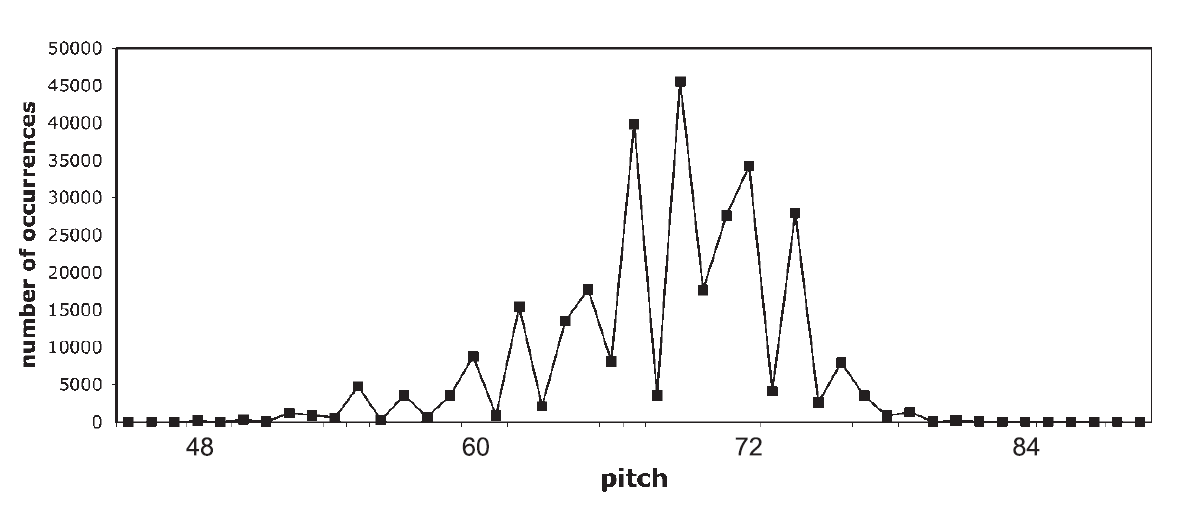
\includegraphics[width=0.75\textwidth]{2_Objectieve_Beoordeling/range}
  \caption{Distributie van alle noten in het Essencorpus.}
  \label{figuur:range}
\end{figure}

Verder is er ook nog de \textit{proximity}, dit heeft te maken met de relatieve afstand tot de voorgaande noot. Bepaalde groottes van sprongen zijn veel waarschijnlijker dan andere. Een sprong met een terts of een kwint komt bijvoorbeeld veel vaker voor dan een sprong van een sext. In het algemeen zijn kleine sprongen veel waarschijnlijker dan grotere. Figuur \ref{figuur:proximity} geeft de frequenties weer waarmee bepaalde intervallen tussen opeenvolgende noten voorkomen in het Essencorpus. \\

\begin{figure}[!ht]
  \centering
  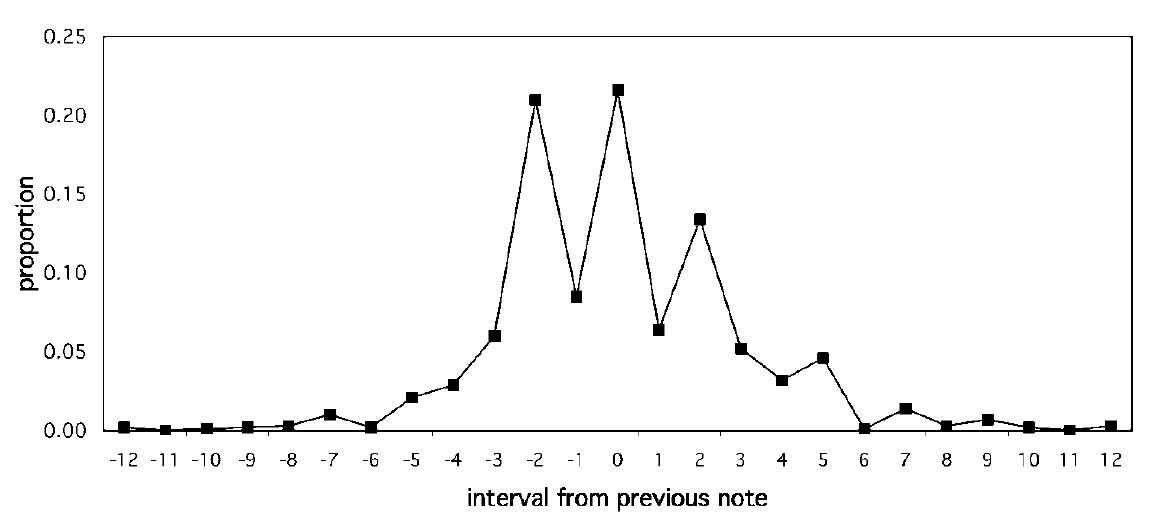
\includegraphics[width=0.75\textwidth]{2_Objectieve_Beoordeling/proximity}
  \caption{Proporties van voorkomen van alle intervallen van opeenvolgende noten in het Essencorpus.}
  \label{figuur:proximity}
\end{figure}

Ten slotte wordt er ook nog rekening gehouden met de \textit{key}, oftewel de toonaard van het muziekstuk. Afhankelijk van de toonaard zijn bepaalde noten waarschijnlijker om voor te komen dan andere. Zo is de grondtoon van een toonladder bijvoorbeeld altijd sterk aanwezig terwijl de noot die een halve toon hoger ligt quasi nooit zal voorkomen in het muziekstuk. Ook is er een verschil in profiel tussen majeur en mineur toonaarden, hier wordt ook rekening mee gehouden. Dit wordt ook ge\"illustreed in figuren \ref{figuur:key_major} en \ref{figuur:key_minor} die resprectievelijk voor stukken die in grote en kleine toonaarden staan de distributies van noten uit het Essencorpus weergeeft. De \textit{range}- en \textit{proximity}-waarden worden gemodelleerd door een normaalverdeling rond respectievelijk de centrale en de vorige noot uit het muziekstuk. De \textit{key}-waarde van een noot wordt bepaald aan de hand van de frequentie van voorkomen van deze zijn nootfunctie in alle muziekstukken van het corpus.

\begin{figure}[!ht]
  \centering
  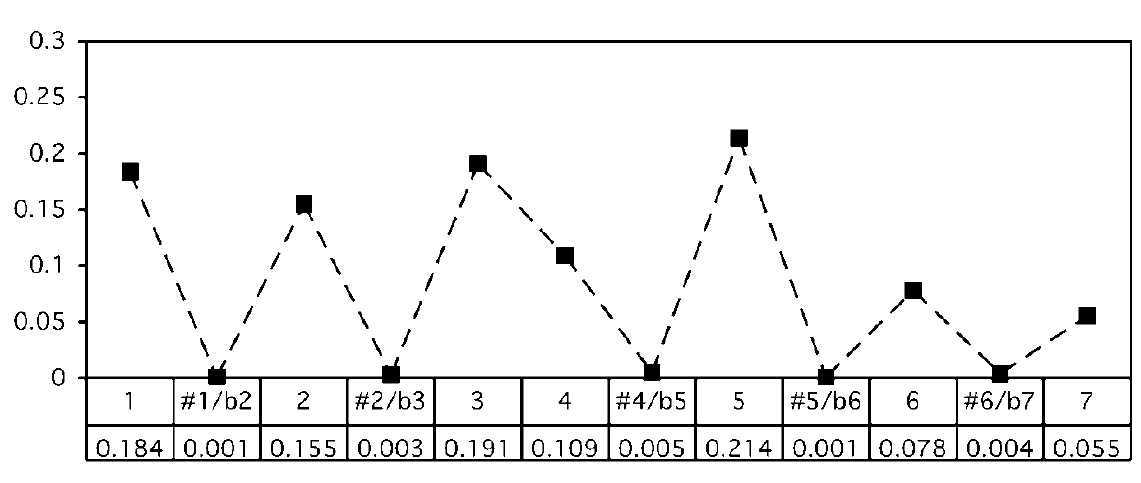
\includegraphics[width=0.75\textwidth]{2_Objectieve_Beoordeling/key_major}
  \caption{Proporties van voorkomen in het Essencorpus van nootfuncties in grote toonladder.}
  \label{figuur:key_major}
\end{figure}

\begin{figure}[!ht]
  \centering
  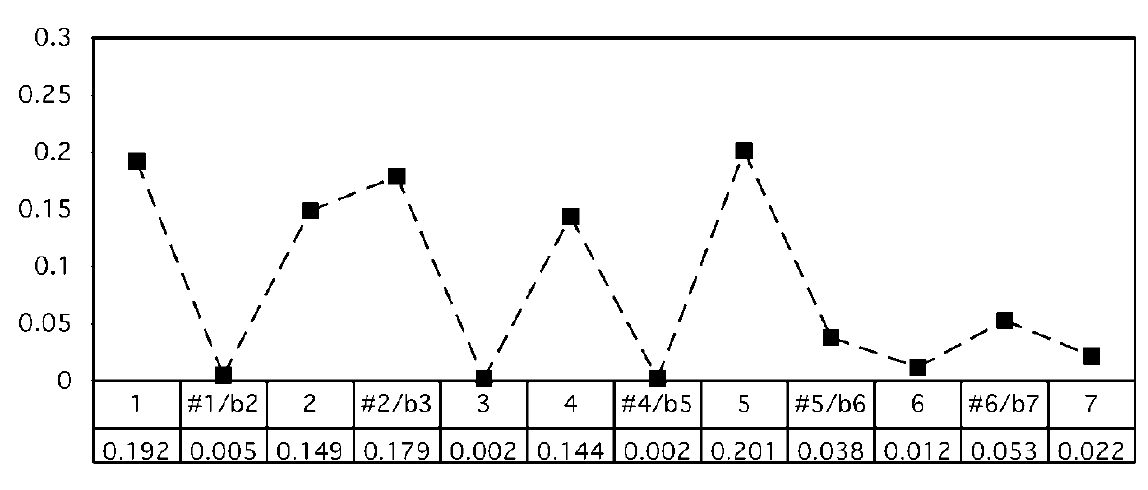
\includegraphics[width=0.75\textwidth]{2_Objectieve_Beoordeling/key_minor}
  \caption{Proporties van voorkomen in het Essencorpus van nootfuncties in kleine toonladder.}
  \label{figuur:key_minor}
\end{figure}

%%% Local Variables: 
%%% mode: latex
%%% TeX-master: "masterproef"
%%% End: 

\chapter{Melodische transformatie}
\label{hoofdstuk:MT}

\section{Inleiding}
In dit hoofdstuk zullen verschillende melodische transformaties besproken worden met hun voor- en nadelen. Deze transformaties zullen werken op melodielijnen die monofoon zijn. Deze melodielijnen zullen behandeld worden als een opeenvolging van noten (toonhoogtes) en het ritme zal na transformatie gewoon behouden blijven. Enkel de toonhoogte van een noot zal aangepast worden. Het ritme zal bij de transformaties die hier besproken staan ook geen invloed hebben op de transformatie van een noot. 

\subsection{Fibonacci}
De transformaties die hier als voorbeeld gegeven worden zullen vaak in een zekere vorm de rij van Fibonacci\cite{url:Fibonacci} bevatten. Dit komt omdat in een vroeg stadium van het onderzoek de vraag bestond of transformaties die voortgaan op de rij van Fibonacci een beter resultaat zouden bieden dan willekeurige transformaties. Dit omdat de rij van Fibonacci in de natuur zo nadrukkelijk aanwezig is dat ook redelijkerwijs de vraag gesteld zou kunnen worden of deze in de muziekwereld zo een invloed zou kunnen hebben. Dit bleek moeilijk hard te maken. Aangezien de resultaten ook zeker niet slechter waren en omdat het ook onderdeel van het onderzoek was, zijn deze transformaties gebaseerd op de rij van Fibonacci vaak gebruikt ter illustratie.

\subsection{Beschrijving van een transformatie}
De melodische transformaties die besproken worden in dit hoofdstuk gaan telkens beschreven worden aan de hand van een tabel. Deze tabel zal telkens een mapping van 8 waarden bevatten. de tweede rij zal altijd waarden tussen -5 en +6 bevatten die als betekenis hebben met welke waarde (namelijk de hoeveelheid halve tonen) een bepaalde noot verhoogd of verlaagd moet worden. 

Welke noot met welke hoeveelheid getransformeerd moet worden wordt dan telkens weergegeven via een waarde op de bovenste rij. Deze rij is ook telkens cyclisch modulo 8. Wanneer bijvoorbeeld zoals in tabel \ref{tabel:transformatie1} de index van de noot weergegeven wordt op de bovenste rij, dan zal de noot op positie 4 met 5 halve tonen verhoogd worden door de transformatie. Maar ook de noot op positie 12 zal met 5 halve tonen verhoogd worden omdat 12 ook 4 geeft als rest na deling door 8.

\subsubsection{Afronding naar de toonaard}
\label{sub:afronding}
In hoofdstuk \ref{OBM:RPK} werd reeds het RPK-model besproken. Dit model wordt gebruikt ter evaluatie van de transformaties. Bij de bespreking van dit model was een van de drie belangrijke kenmerken van een noot om de probabiliteit te bepalen de \textit{key}. Noten die in de toonaard voorkomen zijn zo veel waarschijnlijker om voor te komen dan noten die niet in de toonaard voorkomen. Deze noten, die niet in de toonaard voorkomen, klinken over het algemeen ook vals voor de luisteraar. 

Daarom is ervoor gekozen om na uitvoer van de transformaties nog een afronding door te voeren. Deze afronding bestaat erin om na de transformatie van een noot in de melodielijn, indien deze niet tot de toonaard behoort (en enkel dan), te verhogen of verlagen met een halve toon. De afronding zal zijn naar die noot van de twee die de hoogste probabiliteit heeft volgens het RPK-model. Deze twee noten zullen ook telkens beide wel tot de toonaard behoren. 

De transformaties zelf zullen theoretisch geen rekening houden met deze afronding. Met andere woorden, dit zal niet expliciet vermeld worden in de beschrijvingen van de transformaties. Het is echter wel belangrijk te weten dat dit wel degelijk altijd gebeurt. Vandaar dat het soms ook kan zijn dat het in een illustratie lijkt alsof een transformatie een halve toon the hoog of te laag uitgevoerd is voor een bepaalde noot. Dit ligt dan aan de zonet besproken afronding.

\section{Afbeelding afhankelijk van de positie}
\label{MT:positie}
\subsection{Beschrijving transformatie}
Een eerste, voor de hand liggende melodische transformatie is er eentje die een noot in een muziekstuk gaat transformeren enkel naargelang zijn positie in de melodielijn. De transformatie die ter illustratie dient van dit concept wordt beschreven in tabel \ref{tabel:transformatie1}. Zo zal de noot op positie 6 door deze transformatie met 1 halve toon verhoogd worden. De noot op positie 13 zal met 4 halve tonen verlaagd worden. 

\begin{table}
  \centering
  \begin{tabular}{c | c c c c c c c c }
    Index (mod 8) & 0 & 1 & 2 & 3 & 4 & 5 & 6 & 7 \\
    \hline
    \hline
    Verhoging & 1 & 1 & 2 & 3 & 5 & -4 & 1 & -3 \\
  \end{tabular}
  \caption{Transformatie afhankelijk van de positie van de noot.}
  \label{tabel:transformatie1}
\end{table}

\subsubsection{Voorbeeld}
In figuur \ref{figuur:voorbeeld_transformatie_1} wordt ter illustratie deze transformatie toegepast op een korte melodielijn. De bovenste lijn geeft de originele melodie weer, de onderste lijn geeft het resultaat weer na transformatie. Bij de twee melodielijnen staat bij elke noot telkens ook zijn representatie in halve tonen (modulo 12). Dit zodat het voor de lezer makkelijker te volgen is hoe de transformatie precies verloopt. 

Tussen de twee notenbalken wordt aangegeven welke sprong de transformatie oplegt aan de melodielijn. Zo zal het verschil in getalwaarde tussen overeenkomstige noten op de bovenste en de onderste notenbalk telkens gelijk zijn aan de waarde die hier aangegeven staat. Merk op dat die voor de tweede en zevende noot in dit voorbeeld niet het geval is. Hier lijkt het verschil tussen de noten in de bovenste en onderste lijn telkens een halve toon kleiner dan deze zou moeten zijn. Dit komt door de afronding besproken in onderdeel \ref{sub:afronding} aangezien de noot met getalwaarde 8 (G$\sharp$/A$\flat$) niet tot de toonaard van het muziekstuk (Do groot) behoort.

\begin{figure}[!ht]
  \centering
  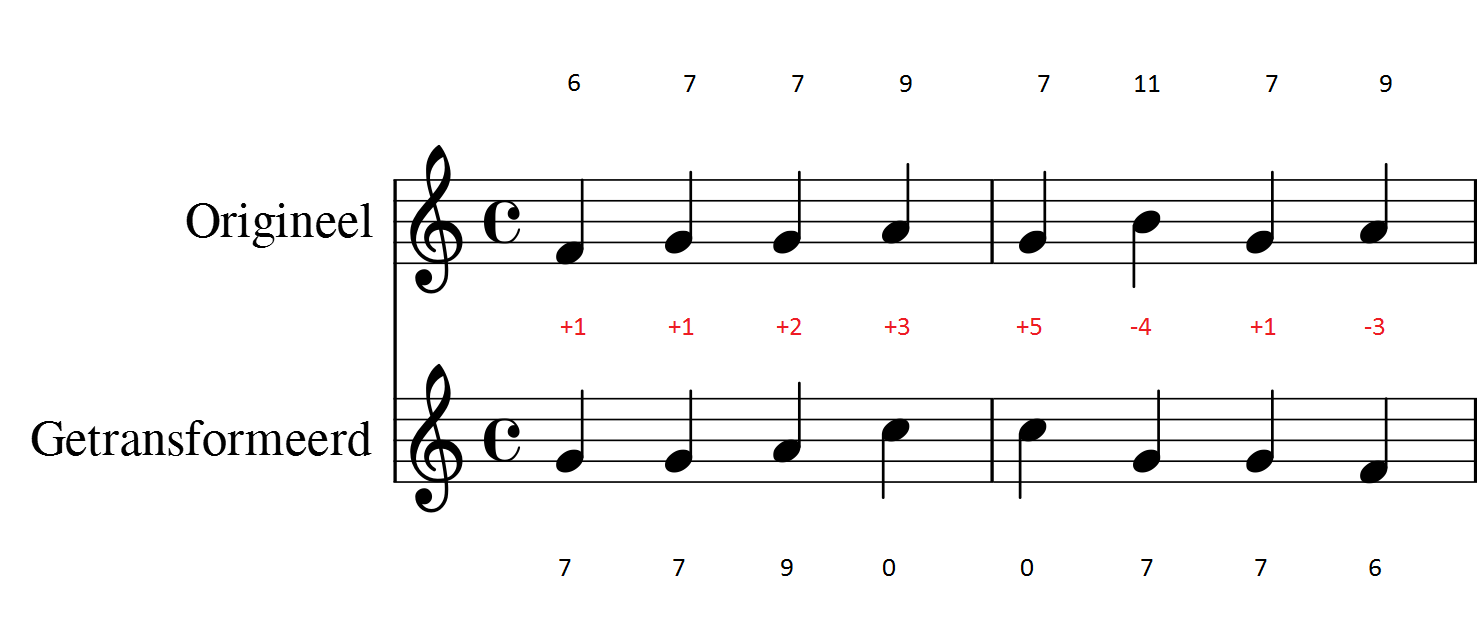
\includegraphics[width=0.75\textwidth]{3_Melodische_Transformatie/transfo1}
  \caption{Voorbeeld van toepassing transformatie afhankelijk van positie.}
  \label{figuur:voorbeeld_transformatie_1}
\end{figure}

\subsubsection{Bespreking transformatie}
Het grootste voordeel van deze transformatie is dat hij zeer eenvoudig uit te voeren en te begrijpen is. Enkel de positie van de noot is van belang met betrekking tot naar welke noot deze getransformeerd zal worden. Een groot nadeel van deze transformatie is dus ook dat deze totaal geen rekening houdt met de eigenlijke toonhoogte van de noot die getransformeerd gaat worden. Er wordt ook geen rekening gehouden met de context van de noot. En als er in het originele stuk patronen zitten zullen die ook nooit herkend en gelijk getransformeerd worden tenzij in het zeer specifieke geval dat deze telkens mooi op een veelvoud van 8 noten van elkaar voorkomen. 

Deze transformatie zal dus ook verder niet veel gebruikt worden. Het kan wel interessant zijn om deze transformatie te zien als een soort van \textit{baseline} voor een willekeurige transformatie, om dan andere transformaties mee te kunnen vergelijken. Ook kan het interessant zijn na te gaan of er veel verschil zit tussen zo een transformaties waarin grote sprongen zitten ten opzichte van transformaties waarin vooral kleinere sprongen zitten (aangezien deze het originele stuk minder zullen gaan vervormen).

\section{Afbeelding afhankelijk van de afstand ten opzichte van vorige noot}
\label{MT:afstand_vorige}
\subsubsection{Beschrijving transformatie}
Een andere melodische transformatie is er een die een noot in een muziekstuk gaat transformeren naargelang zijn afstand ten opzichte van de vorige noot in het muziekstuk. Hierbij zal er gekeken worden naar de afstand van de noot op positie $x$ in de originele melodielijn ten opzichte van de noot op positie $x-1$ in de nieuwe melodielijn (dit is dus de getransformeerde waarde van de vorige noot in het originele muziekstuk). De eerste noot van eender welk muziekstuk wordt in deze transformatie behouden omdat deze noot geen voorgaande noot heeft. 

Wat ook speciaal is aan deze transformatie is dat de verhoging die weergegeven wordt in de transformatietabel toegepast wordt in de tegengestelde richting van waar de huidige noot in de originele melodie staat ten opzichte van de vorige noot na transformatie. De transformatie die ter illustratie dient van dit concept wordt beschreven in tabel \ref{tabel:transformatie2}. 

Zo zal een noot die 2 halve tonen hoger ligt dan de getransformeerde waarde van de vorige noot met 1 halve toon verlaagd worden. Een noot die 6 halve tonen lager ligt dan de getransformeerde waarde van de vorige noot zal met 2 tonen verhoogd worden. Tot slot zal een noot die 1 halve toon lager ligt dan de getransformeerde toonhoogte van de vorige noot nog eens met 4 halve tonen verder verlaagd worden (omdat de waarde in de tabel negatief is).

\begin{table}
  \centering
  \begin{tabular}{c | c c c c c c c c }
    Diff (mod 8) & 0 & 1 & 2 & 3 & 4 & 5 & 6 & 7 \\
    \hline
    \hline
    Verhoging & 5 & -4 & 1 & -3 & 1 & 1 & 2 & 3 \\
  \end{tabular}
  \caption{Transformatie afhankelijk van de afstand van de huidige noot tot de vorige noot na transformatie.}
  \label{tabel:transformatie2}
\end{table}

\subsubsection{Voorbeeld}
In figuur \ref{figuur:voorbeeld_transformatie_2} wordt een voorbeeld gegeven van een korte melodielijn waarop deze transformatie wordt toegepast. Voor de eerste noot wordt er geen transformatie weergegeven, dat is omdat deze ook geen vorige noot heeft en dus niet getransformeerd wordt. 

Als we dan bijvoorbeeld naar de tweede noot kijken dan heeft deze getalwaarde 5, de vorige noot uit de getransformeerde melodie heeft waarde 7 dus het verschil is -2. De absolute waarde is 2 waardoor de sprong als grootte -4 heeft Aangezien het verschil negatief is moet deze waarde bij die van de noot opgeteld worden want we willen een sprong in de richting van de vorige noot. In dit geval zal de sprong toch de andere richting uit gaan aangezien de noot in de tabel zelf negatief is. Zo komen we normaal gezien uit op een noot met getalwaarde 1. Deze noot ligt niet in de toonaard en omdat de noot met getalwaarde 0 (die de grondtoon is van de toonaard) waarschijnlijker is dan die met waarde 2 wordt de noot met waarde 0 als getransformeerde noot gekozen. 

Als we dan verder gaan naar de volgende noot merken we dat het verschil met de getransformeerde van de voorgaande noot 4 halve tonen is. Een absolute waarde van 4 voor het verschil geeft aanleiding tot een sprong van grootte 1. aangezien het verschil positief is en de sprong in tegengestelde richting uitgevoerd moet worden, zal de sprong als waarde -1 hebben. En zo komen we na afronding bij een noot met getalwaarde 4 uit.

\begin{figure}[!ht]
  \centering
  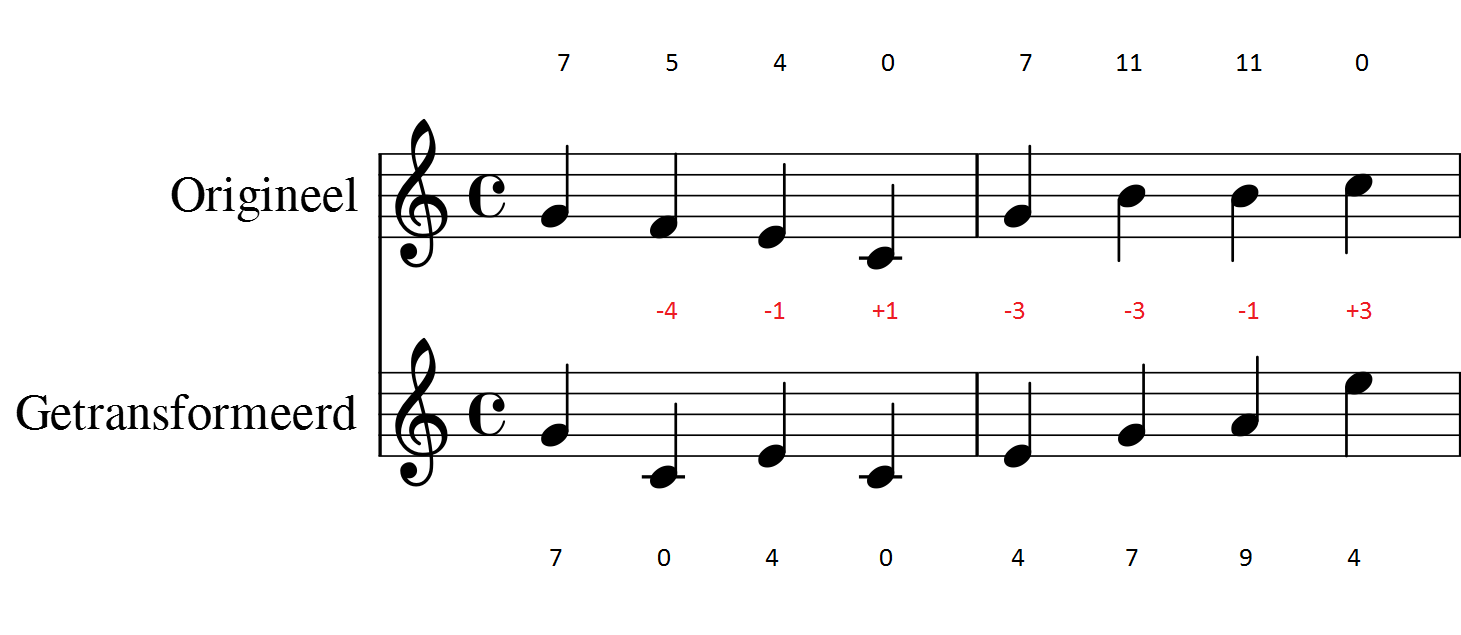
\includegraphics[width=0.75\textwidth]{3_Melodische_Transformatie/transfo2}
  \caption{Voorbeeld van toepassing van de transformatie afhankelijk van het interval ten opzichte van de vorige noot.}
  \label{figuur:voorbeeld_transformatie_2}
\end{figure}

\subsubsection{Bespreking transformatie}
Het interessante aan de transformatie die hier beschreven werd is dat deze de noten niet als losstaand beschouwt, maar ook de context gedeeltelijk in rekening brengt. Dit betekent dat eenzelfde noot naar zeer veel verschillende noten kan getransformeerd worden afhankelijk van de voorgaande noot. 

Een voordeel van deze transformatie is ook dat als er een zekere repetitiviteit in het originele muziekstuk zit, deze bijna altijd ook in het getransformeerde stuk zal voorkomen (enkel de noot die net voor zo een patroon voorkomt kan nog een extra invloed hebben). Dit maakt dat de structuur van het originele stuk nog iets meer bewaard blijft. 

Een nadeel van deze transformatie is dat deze wel nog steeds blind is voor de rest van de context. Ook de toonhoogte van de noot zelf heeft geen invloed op de grootte en richting van de transformatie op deze noot.  

%%% Local Variables: 
%%% mode: latex
%%% TeX-master: "masterproef"
%%% End: 

\chapter{Effici\"ent Toepassen Transformatie}
\label{hoofdstuk:ETT}

In dit hoofdstuk worden twee algoritmes behandeld die varianten zijn van elkaar. In beide algoritmes is het de bedoeling om een gegeven muziekstuk te transformeren tot een nieuw muziekstuk op zo een manier dat de totale consonantiescore zo hoog mogelijk is. Dit kan gebeuren door een aantal toegelaten operaties op het oorspronkelijke muziekstuk. Buiten de originele melodielijn zullen namelijk ook een aantal verschillende transformaties (zoals die beschreven zijn in onderdeel \ref{MT:afstand_vorige}) meegegeven worden aan het algoritme. Deze transformaties zullen door het algoritme gebruikt worden om het originele stuk te transformeren naar een nieuw stuk met een hogere score. Voor elke noot van de melodielijn heeft het algoritme namelijk de keuze om ofwel de noot te behouden, ofwel deze te transformeren conform een van de transformaties die meegegeven werden aan het algoritme. Het algoritme dat hier voor zorgt wordt beschreven in onderdeel \ref{ETT:algo1}. In gedeelte \ref{ETT:algo2} wordt een algoritme beschreven dat eenzelfde doel heeft maar een extra voorwaarde opgelegd krijgt. Deze voorwaarde stelt dat als met een transformatie wilt toepassen, men telkens een minimum aantal opeenvolgende noten moet transformeren met deze transformatie. 

\section{Beste sequentie}
\label{ETT:algo1}

\subsection{Doelstelling}
Het algoritme dat hier beschreven wordt is afhankelijk van twee parameters. Een eerste parameter is een originele melodielijn. De tweede parameter beschrijft een aantal transformaties (gedifini\"eerd zoals in onderdeel \ref{MT:afstand_vorige}), die gebruikt mogen worden door het algoritme. Het doel is nu om gebruik makend van enkel deze verschillende mogelijke transformaties de originele melodielijn te transformeren tot de nieuwe melodielijn die de hoogste consonantiescore oplevert. Hierbij heeft het algoritme voor elke noot in het muzikstuk twee mogelijke keuzes. Een eerste mogelijkheid is dat de noot niet getransformeerd wordt en identiek overgenomen wordt in de nieuwe melodielijn. De tweede mogelijkheid bestaat erin dat de noot ook getransformeerd mag worden, maar denk enkel volgens een van de beschikbare transformaties.

\subsection{Idee van het algoritme}
Een eerste belangrijke observatie is dat eender welke noot in het muziekstukje zelf op slechts maximaal 14 verschillende noten kan afgebeeld worden. Elke noot kan namelijk door transformatie enkel afgebeeld worden op een noot die maximaal 5 halve tonen lager ligt dan de oorspronkelijke noot en ook maximaal 6 halve tonen hoger ligt dan de originele noot (dit is een deel van de definitie van de soort transformaties die gebruikt worden in het algoritme). Er is nu echter nog een speciaal geval waarbij een transformatie tot een van de twee extreme gevallen zou leiden en deze noot dan ook nog eens geen deel zou uitmaken van de tonaard. In dat geval is het mogelijk dat de noot nog een halve toon verder afgerond wordt om terug tot op een noot te komen die in de toonaard ligt. Elke noot kan dus theoretisch gezien (na afronding) afgebeeld worden op eender welke noot die maximaal 6 halve tonen lager en maximaal 7 halve tonen hoger ligt dat zichzelf. Dit zijn in totaal 14 verschillende mogelijkheden.\\
Het belangrijkste idee van het algoritme is gebaseerd op de principes van \textit{dynamic programming} \cite{url:DP}. Bij dit algoritme komt het er op neer dat achtereenvolgens voor elke noot in het muziekstuk het best pad (en bijhorende beste score) bijgehouden zal worden voor elk van de 14 mogelijke toonhoogtes die deze noot kan aannemen in de nieuwe melodielijn. En enkel op deze optimale paden zal verder gerekend worden om te bepalen wat de beste paden zijn tot de 14 mogelijke toonhoogtes die de volgende noot in het muziekstuk kan aannemen. Dit wordt dan verder herhaald tot alle noten van de originele melodielijn overlopen zijn.

\subsection{Werking van het algoritme}
In dit onderdeel zal de werking van het algoritme beschreven worden. Als extra referentie voor de lezer is de broncode bijgevoegd in appendix \ref{Broncode:algo1}.\\ 
Het algoritme zal tijdens de uitvoering gebruik maken van 3 hulpvariabelen. De eerste twee van deze hulpvariabelen zijn eendimensionale arrays van lengte 14. De eerste array, die de naam \textit{past} meekrijgt, stelt de probabiliteiten voor van de beste paden eindigend bij alle mogelijke noten waarnaar de vorige beschouwde noot kan getransformeerd worden. De tweede array, die \textit{current} genoemd wordt, bevat de probabiliteiten van de beste paden die eindigen op de huidig beschouwde noot (of een van zijn mogelijke transformaties). De waarden in deze twee arrays, zullen in het algoritme niet de probabiliteiten zelf, maar hun logaritmen zijn, dit om het rekenwerk te vereenvoudigen. De derde hulpvariabele, \textit{matrix}, is een tweedimensionale array en heeft een dimensie van de lengte van de melodielijn op 14. Deze variabele gaat voor elke mogelijke waarde die elke noot in het muziekstukje kan aannemen, weergeven vanwaar het beste pad komt dat eindigt bij deze noot.\\
Om de betekenis van deze variabelen nog iets concreter te maken zal gebruik gemaakt worden van de volgende notatie. De letter `C' voor de toonhoogte van de huidig beschouwde noot in de originele melodielijn. De letter `P' voor de toonhoogte van de vorige noot in het originele muziekstukje. Zo zal de waarde C+3 staan voor de noot met een toonhoogte die drie halve tonen hoger ligt dan de huidige noot in het originele stukje. P-4 zal dan bijvoorbeeld staan voor de noot met een toonhoogte die 4 halve tonen lager ligt dan de vorige noot in de originele melodielijn. Verder zal, er als er in gesproken wordt over de i-de noot in het muziekstuk, de noot op positie i bedoeld worden. Zo zal de 0-de noot in het muziekstukje de eerste noot zijn, de 1-de noot zal de tweede noot van het muziekstukje zijn enzovoort.\\ 
Stel we beschouwen momenteel de n-de noot van het muziekstukje. Dan zullen volgende stellingen gelden. Op positie \textit{past[i]} zal de waarde voor de probabiliteit staan van het beste pad van n noten dat eindigt op de noot `P+i-6'. Ook zal tijdens uitvoering van het algoritme de \textit{current} array aangepast worden. Met als doelstelling: op positie \textit{current[i]} zal de waarde voor de probabiliteit berekend worden voor het beste pad van (n+1) noten dat eindigt op de noot `C+i-6'. De waarde van het element matrix[i][j] verwijst naar vanwaar het beste pad komt van (n+1) noten dat eindigt op de noot `C+j-6'. Stel nu dat matrix[i][j]=k, dan betekent dit dat het beste pad van (n+1) noten dat eindigt op noot `C+j-6', een verlenging is van het beste pad van n noten dat eindigt op noot `P+k-6'. 

\subsubsection{Initialisatie}
De eeste stap in het algoritme zal de noot op positie 1 als huidige noot bekijken en de noot op positie 0 als vorige noot. De hulpvariabelen moeten dus ge\"initialiseerd worden zodat ze daaraan voldoen. Hierdoor zal de array \textit{past} voor al zijn posities een hele lage waarde meekrijgen (-100 als logaritme van de probabiliteit in de broncode weergegeven in appendix \ref{Broncode:algo1}) behalve voor de noot op positie 6. Deze noot staat namelijk voor dezelfde noot als oorspronkelijke noot en aangezien de oorspronkelijke noot op positie 0 nooit getransformeerd wordt, zal \textit{past[6] = 0}. Dit betekent dat dat kans op het behouden van de eerste noot gelijk is aan 1. De \textit{current} array krijgt voor al zijn posities zeer lage waarden mee. De bedoeling hiervan is dat eender welk pad dat als eerste gevonden wordt dat voortgaat op de vorige noot een hogere probabiliteit zal hebben dan deze waarde. Tot slot zal ook elke waarde van \textit{matrix} op een arbitraire startwaarde 0 gezet worden. De waarde die hier in het begin gezet wordt is van geen belang, aangezien deze waarden toch overschreven zullen worden wanneer de beste paden berekend worden.

\subsubsection{Een stap in het algoritme}
Voor elke noot in het muziekstukje, beginnend vanaf de noot op positie 1, zal nu het volgende uitegevoerd worden. Stel ook dat we momenteel als huidige noot, de noot op positie n beschowen.\\ 
Allereerst gaan we op \textit{current[6]} de waarde zetten van het beste pad dat de huidige noot niet transformeert. Om dit te doen gaan we kijken naar de probabiliteiten van de beste paden die eindigen op alle 14 mogelijke noten die als vorige noot zouden kunnen doorgaan. Deze probabiliteiten staan uiteraard gewoon in \textit{past}. Voor elk element \textit{past[i]} wordt nu zijn waarde bij de afstandsprobabiliteit ten opzichte van de huidig beschouwde noot opgeteld. Als deze waarde hoger is dan de huidige beste waarde van \textit{current[6]}, dan wordt de waarde van \textit{current[6]} overschreven en wordt de waarde \textit{matrix[n][6]} op i gezet.
Als tweede stap gaan we voor elke mogelijk transformatie kijken naar welke noot de noot op `P+i-6' de noot huidige noot gaat afbeelden. En dit voor alle 14 mogelijke vorige noten. Stel nu dat de noot `P-i+6' de huidig beschouwde noot afbeeldt op noot `C+j-6'. Als nu de de som van \textit{past[i]} en de afstandsprobabiliteit tussen deze twee noten groter is dan de huidige waarde \textit{current[j]}, dan zal deze waarde overschreven worden. Alsook zal \textit{matrix[n][j]} gelijk gesteld worden aan i. Dit aangezien het nieuwe meest waarschijnlijke pad dat gevonden is dat eindigt op `C+j-6', komt van de noot `P+i-6'.\\
Wanneer dit uitgevoerd is, bevat \textit{current} de probabiliteiten van de beste paden van lengte (n+1) die eindigen op de 14 mogelijke toonhoogtes waarop de huidig beschouwde noot kan afgebeeld worden.
Het enige wat nu nog rest is om de waarden van \textit{current} over te zetten naar \textit{past}. En om \textit{current} daarna terug te initialiseren op zeer lager waarden. Dit zodat de arrays klaar zijn voor het beschouwen van de volgende noot in het muziekstukje. 

\subsubsection{Extractie van het beste pad}
Na uitvoeren van het vorige gedeelte voor elke noot in het muziekstukje zal \textit{past} de probabiliteiten bevatten van de beste paden voor elk van de 14 mogelijke eindnoten van het geheel van het nieuwe muziekstukje. Als eerste zal er dus gekeken worden welke van deze 14 toonhoogtes het meest waarschijnlijke pad heeft. Dit pad is het pad dat we zoeken in dit algoritme. Het enige wat nu nog rest is om vanaf dit punt dat pad te reconstueren. Dit gebeurt met behulp van de \textit{matrix} array. Beginnen bij de laatste noot en zo opschuivend terug naar voor wordt hiervoor het volgende gedaan. Stel we zitten bij noot n. Noem `C+i-6' de toonhoogte van de huidige noot die in dit beste pad zit. Noem nu \textit{matrix[n][i]} = j. Dan is de vorige noot van het optimale pad de noot met als toonhoogte `P+j-6', waarbij P de toonhoogte is van de overeenkomstige noot in het originele muziekstuk. \textit{matrix[n-1][j]} geeft dan weer aanleiding tot de noot die daarvoor staat in het optimale pad, enzovoort. Op deze manier kan het volledige optimale pad weer gereconstrueerd worden.

\subsection{Performantie en geheugencomplexiteit}
De parameters waarvan het algoritme afhankelijk is, zijn de lengte van de melodielijn in de invoer en ook het aantal transformaties (in het voorbeeld beschreven in appendix \ref{Broncode:algo1} wordt gebruik gemaakt van slechts 2 transformaties, maar het algoritme werkt voor eender welk aantal transformaties dat gedefini\"eerd wordt).\\ 
De snelheid van het algoritme is lineair afhankelijk van beide van deze parameters. Indien de lengte van het originele melodietje met een factor f omhoog gaat en de rest constant blijft dan gaat ook het aantal stappen in het algoritme met een factor f omhoog. Het rekenwerk per stap blijft echter gelijk. Wanneer het aantal transformaties met een factor f omhoog gaat en de rest constant blijft, dan zal het aantal stappen onveranderd blijven. Het rekenwerk per stap gaat wel met een factor f omhoog (op het constante rekenwerk per stap van het `niet transformeren' na).\\
Het geheugen dat nodig is voor de uitvoer van het algoritme is lineair afhankelijk van de lengte van de originele melodie. Dit komt omdat de \textit{matrix} array als een van zijn dimensies deze lengte heeft. Wanneer de lengte van het originele stukje met een factor f omhoog gaat, zal de grootte van deze array dus ook met een factor f omhoog gaan. De grootte van de andere twee gebruikte arrays tijdens de uitvoer van het algoritme is onveranderlijk ten opzichte van die lengte. Maar in het total geheugengebruik is de \textit{matrix} array dominant aangezien deze zo veel groter is. Het aantal gebruikte transformaties heeft geen effect op het geheugengebruik van het algoritme.

\section{Beste sequentie met minimum transformatie lengte}
\label{ETT:algo2}

\subsection{Doelstelling}
Het algoritme dat in dit onderdeel beschreven wordt heeft dezelfde doelstelling als het algoritme beschreven in onderdeel \ref{ETT:algo1}. Enkel wordt dit algoritme aan nog een extra restrictie onderworpen. Zo zal dit algoritme afhankelijk zijn van drie parameters. De eerste twee parameters zijn een originele melodielijn en een aantal toegelaten transformaties. Als extra parameter is dit algoritme nog afhankelijk van een opgegeven minimum transformatie lengte. Dit betekent dat het algoritme enkel een deel van de originele melodielijn mag transformeren als hij voor minstens dit opgegeven aantal opeenvolgende noten dezelfde transformatie toepast. Er zijn een aantal overeenkomsten tussen dit algoritme en het algoritme beschreven in sectie \ref{ETT:algo1}. Bij het bespreken van deze overeenkomsten zal er verwezen worden naar overeenkomstige delen in dat hoofdstuk. Daar waar dit algoritme verschilt van het vorige zal een volledige uitleg gegeven worden.

\subsection{Idee van het algoritme}
Ook nu zal er gebruik gemaakt worden van de principes van \textit{dynamic programming}. Dit zal enkel op een verschillende manier gebeuren dan bij het vorige algoritme, aangezien de opgegeven minimumlengte verhindert om eenzelfde data representatie te gebruiken, waarom dit precies noodzakelijk is wordt verder in de tekst nog verduidelijkt. Het idee van dit algoritme bestaat erin om elke noot van het muziekstukje chronologisch te overlopen. En bij elke noot uit het originele stuk zijn er dan een aantal mogelijkheden om het beste pad te bepalen dat eindigt op een van de 14 mogelijke noten waarin de originele noot kan getransformeerd worden. Als in het vervolg van de tekst gesproken wordt over een `geldig pad', dan wordt hier een pad mee bedoeld dat de regels van de minimumlengte voor transformatie en de mogelijke transformaties respecteert. De parameter die voor de minimum transformatie lengte staat wordt met `ML' aangeduid. Een eerste mogelijkheid voor zo een optimaal pad is de uitbreiding van eender welk optimaal pad dat eindigt bij de vorige noot met het behouden van de huidige noot. Een tweede mogelijkheid is het uitbreiden van een optimaal pad dat geldig is, eindigt op de vorige noot en eindigt met transformatie f (en dus minstens zijn ML laatste noten met die transformatie is bekomen aangezien we al stelden dat het pad geldig was) uit te breiden met weer dezelfde transformatie f. Tot slot is er ook nog de mogelijkheid om eender welk optimaal en geldig pad van lengte ML korter dan het huidige uit te breiden met ML keer dezelfde transformatie. Op deze manier kunnen alle optimale paden bekomen worden die aan de vooropgestelde eisen voldoen.

\subsection{Werking van het algoritme}
In dit onderdeel zal de werking van het algoritme beschreven worden. Als extra referentie voor de lezer is de broncode bijgevoegd in appendix \ref{Broncode:algo2}.\\
Tijdens de uitvoering van het algoritme worden er 8 hulpvariabelen (allemaal arrays) gebruikt die hieronder opgelijst worden, met korte uitleg over hun betekenis.

\begin{itemize}
    \item \textbf{prob \textunderscore keep \textunderscore past:} Houdt de probabiliteiten bij voor de optimale 	en geldige paden die eindigen op een van de laatste ML bekeken noten. En dit 		enkel voor de paden die eindigen zonder transformatie van de laatste noot.
    \item \textbf{prob \textunderscore keep \textunderscore current:} Houdt de probabiliteit bij voor het optimaal en geldig pad dat eindigt op de huidig beschouwde noot. En dit enkel voor de paden die eindigen zonder transformatie van hun laatste noot.
    \item \textbf{prob \textunderscore transform \textunderscore past:} Houdt voor elke toegelaten transformatie afzonderlijk de probabiliteiten bij voor de optimale en geldige paden die eindigen met deze transformatie. En dit voor al zo een paden die eindigen op een mogelijke transformatie van een van de laatste ML beschouwde noten.
    \item \textbf{prob \textunderscore transform \textunderscore current:} Houdt voor elke toegelaten transformatie afzonderlijk de probabiliteiten bij voor de optimale en geldige paden die eindigen met deze transformatie. En dit voor al zo een paden die eindigen op de huidig beschouwde noot.
    \item \textbf{path \textunderscore end \textunderscore on \textunderscore keep \textunderscore past:} Houdt de optimale en geldige paden bij die horen bij de probabiliteiten weergegeven in \textit{prob \textunderscore keep \textunderscore past}.
    \item \textbf{path \textunderscore end \textunderscore on \textunderscore keep \textunderscore current:} Houdt het optimale pad bij dat hoort bij de probabiliteit weergegeven in \textit{prob \textunderscore keep \textunderscore current}.
    \item \textbf{prob \textunderscore end \textunderscore on \textunderscore transform \textunderscore past:} Houdt de optimale en geldige paden bij, horende bij de probabiliteiten van \textit{prob \textunderscore transform \textunderscore past}.
    \item \textbf{prob \textunderscore end \textunderscore on \textunderscore transform \textunderscore current:} Houdt de optimale en geldige paden bij, horende bij de probabiliteiten van \textit{prob \textunderscore transform \textunderscore current}.
\end{itemize}

\subsubsection{Initialisatie}
\subsubsection{Een stap in het algoritme}
\subsubsection{Extractie van het beste pad}

\subsection{Performantie en geheugencomplexiteit}

%%% Local Variables: 
%%% mode: latex
%%% TeX-master: "masterproef"
%%% End: 

\chapter{Experimenten en Resultaten}
\label{hoofdstuk:ER}
In dit hoofdstuk worden de belangrijkste experimenten besproken die uitgevoerd in het verloop van deze masterproef. Deze hebben zowel betrekking op de besproken melodische transformaties, de algoritmes om deze transformaties te combineren en ook het RPK-model dat gebruikt werd om deze transformaties te evalueren.\\
De resultaten worden meestal weergegeven op een plot waarbij op de y as de gemiddelde probabiliteit staat. Deze probabiliteit staat voor de gemiddelde probabiliteit van voorkomen van een noot (gegeven de vorige noot) volgens het RPK-model in alle muziekstukken waarop er getest werd. Als er dus in dit hoofdstuk gesproken wordt over een gemiddelde probabiliteit van een bepaald muziekstuk dan betekent dit de gemiddelde probabiliteit van een noot in dit muziekstuk.

\section{Experimenten met melodische transformaties}
\subsection{Vergelijking van de twee melodische transformaties}
\label{experiment:5}
\subsubsection{Beschrijving experiment}
Dit experiment heeft als opzet om de twee verschillende soorten transformaties die besproken werden in hoofdstuk \ref{hoofdstuk:MT} te vergelijken in performantie. De eerste transformatie gaat een noot in de melodielijn transformeren naargelang zijn positie in de notensequentie (deze transformatie noemen we in het vervolg van die onderdeel T1). De tweede transformatie gaat een noot transformeren enkel op basis van zijn (melodische) afstand ten opzichte van de vorige noot in de melodielijn (deze transformatie noemen we in de rest van dit onderdeel T2). De werking van deze twee transformaties staat beschreven respectievelijk in hoofdstukken \ref{MT:positie} en \ref{MT:afstand_vorige}.

Voor dit experiment zullen voor 50 testgevallen telkens 10 verschillende willekeurige voorkomens voor beide transformatie getest worden. Zo een willekeurige transformatie wordt bekomen door 8 opeenvolgende getallen tussen -5 en +6 (beide grenzen inclusief) willekeurig te genereren. Noem deze 8 getallen in volgorde $X_{i}$ met 0$\leq$ i$\leq$ 7. Voor T1 levert dit dan de transformatie op beschreven in tabel \ref{tabel:exp5:T1}, voor T2 levert dit de transformatie beschreven in tabel \ref{tabel:exp5:T2}.

\begin{table}
  \centering
  \begin{tabular}{c | c c c c c c c c }
    Pos (mod 8) & 0 & 1 & 2 & 3 & 4 & 5 & 6 & 7 \\
    \hline
    \hline
    Verhoging & $X_{0}$ & $X_{1}$ & $X_{2}$ & $X_{3}$ & $X_{4}$ & $X_{5}$ & $X_{6}$ & $X_{7}$ \\
  \end{tabular}
  \caption{Willekeurige transformatie volgens T1, gebruikt in het experiment van onderdeel \ref{experiment:5}.}
  \label{tabel:exp5:T1}
\end{table}

\begin{table}
  \centering
  \begin{tabular}{c | c c c c c c c c }
    Diff (mod 8) & 0 & 1 & 2 & 3 & 4 & 5 & 6 & 7 \\
    \hline
    \hline
    Verhoging & $X_{0}$ & $X_{1}$ & $X_{2}$ & $X_{3}$ & $X_{4}$ & $X_{5}$ & $X_{6}$ & $X_{7}$ \\
  \end{tabular}
  \caption{Willekeurige transformatie volgens T2, gebruikt in het experiment van onderdeel \ref{experiment:5}.}
  \label{tabel:exp5:T2}
\end{table}

Voor elk van de 50 testgevallen worden zo dus 20 transformaties gegenereerd (10 voor T1 en 10 voor T2). Over deze 50 testgevallen en 10 transformaties per transformatie soort wordt dan een gemiddelde consonantiescore berekend. De exponenti\"ele van deze consonantie score levert dan voor beide transformatie soorten een gemiddelde probabiliteit van een getransformeerd muziekstuk.

\subsubsection{Resultaten}

\begin{table}
  \centering
  \begin{tabular}{c | c c }    
    Transformatie & Consonantiescore & Probabiliteit(\%)\\
    \hline
    Oiginele melodie & -2.36 & 9.42\\
    T1 & -3.72 & 2.43\\
    T2 & -3.19 & 4.12\\
  \end{tabular}
  \caption{Resulaten van experiment \ref{experiment:5}. Gemiddelde consonantiescores voor de twee soorten transformaties en de originele melodielijnen die getranformeerd werden. De twee geteste soorten van transformaties staan beschreven in onderdelen \ref{MT:positie}(T1) en \ref{MT:afstand_vorige}(T2).}
  \label{tabel:res5}
\end{table}

In tabel \ref{tabel:res5} staan de resultaten van dit experiment weergegeven. Er valt meteen op dat beide transformaties de originele melodielijnen gemiddeld gezien transformeren naar een nieuwe melodielijn met een minder goede consonantiescore. Er is ook een duidelijk verschil merkbaar in kwaliteit van de transformaties, T2 scoort merkbaar beter dan T1. Dit is ook logisch aangezien T1 eigenlijk niets van informatie over het muziekstuk in rekening brengt, buiten zijn absolute positie (modulo 8). T2 brengt de afstand tot de vorige noot in rekening wat er toe kan leiden dat in sommige gevallen de intervallen tussen opeenvolgende noten relatief kleiner gehouden wordt dan bij T1, wat consistenter betere scores kan opleveren volgens het RPK-model.

\subsection{Vergelijking Fibonacci transformatie met gemiddelde transformatie}
\label{experiment:6}
\subsubsection{Beschrijving experiment}
Het doel van dit experiment is om na te gaan of een transformatie, die gebaseerd is op de rij van Fibonacci een beter resultaat geeft dan een gemiddelde transformatie. De reden dat er specifiek getest wordt op de rij van Fibonacci is omdat deze bekende rij in zoveel verschillende onderdelen van de natuur te herkennen valt dat het in zeker zin niet onlogisch zou zijn, moest deze ook in de muziek onder bepaalde vormen voorkomen. Voor beide soorten van transformaties die beschreven staan in onderdelen \ref{MT:positie} en \ref{MT:afstand_vorige} (en die we in het kort respectievelijk T1 en T2 noemen), wordt zo een transformatie gecre\"eerd die gebaseerd is op de rij van fibonacci. Deze transformaties worden beschreven door tabellen \ref{tabel:exp6:T1} en \ref{tabel:exp6:T2}. Hierbij is elk getal op de onderste rij telkens de gelijk aan het overeenkomstig element uit de rij van fibonacci modulo 12, waarbij de waarde van elke sprong tussen -5 en +6 ligt.

\begin{table}
  \centering
  \begin{tabular}{c | c c c c c c c c }
    Positie (mod 8) & 0 & 1 & 2 & 3 & 4 & 5 & 6 & 7 \\
    \hline
    \hline
    Verhoging & 1 & 1 & 2 & 3 & 5 & -4 & 1 & -3 \\
  \end{tabular}
  \caption{Fibonacci transformatie volgens T1 gebruikt in het experiment van onderdeel \ref{experiment:6}.}
  \label{tabel:exp6:T1}
\end{table}

\begin{table}
  \centering
  \begin{tabular}{c | c c c c c c c c }
    Diff (mod 8) & 0 & 1 & 2 & 3 & 4 & 5 & 6 & 7 \\
    \hline
    \hline
    Verhoging & 1 & 1 & 2 & 3 & 5 & -4 & 1 & -3 \\
  \end{tabular}
  \caption{Fibonacci transformatie volgens T2 gebruikt in het experiment van onderdeel \ref{experiment:6}.}
  \label{tabel:exp6:T2}
\end{table}

Nu wordt op dezelfde 50 testgevallen als waarop getest werd in experiment \ref{experiment:5}, deze twee transformaties toegepast. De gemiddelde consonantiescores die deze twee Fibonacci transformaties opleveren kunnen nu vergeleken worden met het gemiddelde algemene geval voor de twee soorten transformaties. 

\subsubsection{Resultaten}

\begin{table}
  \centering
  \begin{tabular}{c | c c }    
    Transformatie & Consonantiescore & Probabiliteit(\%)\\
    \hline
    Oiginele melodie & -2.36 & 9.42\\
    T1 & -2.92 & 5.42\\
    T2 & -2.63 & 7.21\\
  \end{tabular}
  \caption{Resulaten van experiment \ref{experiment:6}. Gemiddelde consonantiescores voor de twee Fibonacci transformaties en de originele melodielijnen die getranformeerd werden.}
  \label{tabel:res6}
\end{table}

Tabel \ref{tabel:res6} geeft de resultaten van de Fibonacci transformaties weer. In tabel \ref{tabel:res5} staan de resultaten van dezelfde soorten transformaties maar dan met willekeurige sprongen in plaats van sprongen volgens de rij van Fibonacci. Er valt op dat voor beide transformatie soorten, de transformatie volgens de rij van Fibonacci merkbaar beter scoort dan een gemiddelde transformatie van zijn soort. Een reden hiervoor is dat de sprongen in de Fibonacci transformaties redelijk klein zijn (bijvoorbeeld drie keer op acht een sprong van slechts een halve toon). Hierdoor zal het originele muziekstuk minder aangepast worden en de score dus ook niet zo veel verslechteren dan na een gemiddelde transformatie. 

Voor de Fibonacci transformatie volgens T2 kan zelfs gezegd worden dat deze zeer goed scoort, aangezien de consonantiescore die gemiddeld bekomen wordt met deze transformatie zelfs in de buurt ligt van de originele melodielijn. De reden hiervoor is dat er bij deze transformatie veel dezelfde noten na elkaar gecre\"eerd worden (wat goede scores geeft voor het RPK-model aangezien de \textit{proximity} maximaal is). Dit komt doordat sprongen in dit algoritme in tegengestelde richting uitgevoerd worden als de afstand ten opzichte van de vorige noot. En afstanden van grootte 1, 2 en 3 worden bijvoorbeeld allemaal gecounterd door een sprong van dezelfde grootte in tegengestelde richting. Hierdoor zullen noten die op zo een afstand van elkaar zitten telkens op dezelfde noot afgebeeld worden.

Er kan dus besloten worden dat deze Fibonacci transformaties iets betere resultaten leveren dan een gemiddelde transformatie (wat de consonantiescore betreft). Dit betekent echter niet automatisch dat de muziekstukken ook beter klinken want bijvoorbeeld bij de Fibonacci transformatie volgens tabel \ref{tabel:exp6:T2} zullen sequenties gecre\"eerd worden die veel dezelfde noten bevatten, wat over het algemeen niet als interessante muziek beschouwd wordt.

\section{Experimenten met het RPK-model}
\subsection{Afhankelijkheid score RPK-Model en gemiddelde afstand tussen opeenvolgende noten}
\label{experiment:10}
\subsubsection{Beschrijving experiment}
De bedoeling van dit experiment is om na te gaan hoe sterk het verband is tussen de consonantiescore van een muziekstuk en de gemiddelde afstand tussen opeenvolgende noten in datzelfde muziekstuk. De reden dat deze test wordt gedaan is om dat de afstand tot de vorige noot een belangrijke parameter is in de berekening van de consonantiescore volgens het RPK-model. Indien er een sterke afhankelijkheid zou zijn dan kan de gemiddelde afstand tot opeenvolgende noten in een muziekstuk als een soort eerste voorspeller dienen voor de consonantiescore die computationeel veel minder zwaar is dan de berekening van de consonantiescore zelf.

Voor dit experiment wordt voor 100 muziekstukken uit het Essencorpus de consonantiescore berekend alsook de gemiddelde afstand tussen twee opeenvolgende noten. Hierna wordt de absolute waarde van de consonantiescore uitgezet ten opzichte van de gemiddelde afstand. 

\subsubsection{Resultaten}
\begin{figure}[!ht]
  \centering
  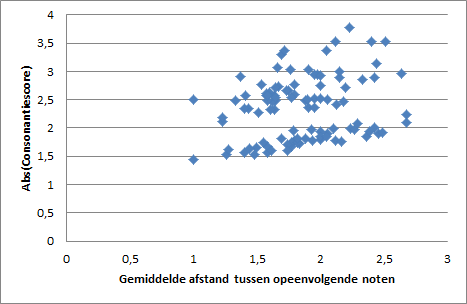
\includegraphics[width=0.75\textwidth]{5_Experimenten_Resultaten/exp10_res}
  \caption{Resultaten van het experiment uitgevoerd in deel \ref{experiment:10}. Absolute waarde van de consonantiescore uitgezet t.o.v. de gemiddelde afstand in halve tonen tussen opeenvolgende noten in het muziekstuk.}
  \label{figuur:exp10}
\end{figure}

De resulaten van dit experiment staan weergegeven in figuur \ref{figuur:exp10}. op de y-as staat de absolute waarde van de consonantiescore gegeven, een lagere score komt hierbij overeen met een hogere probabiliteit van het muziekstuk volgens het RPK-model. Op de figuur is er een verband zichtbaar waarbij een hogere gemiddelde afstand tussen opeenvolgende noten gemiddeled gezien ook leidt tot een hogere absolute waarde voor de consonantiescore (en dus een lagere probabiliteit voor het muziekstuk). Het verband is echter niet sterk genoeg om de afstand tussen opeenvolgende noten als nuttige voorspeller te zien voor de consonantiescore van een muziekstuk.

\subsection{Afhankelijkheid score RPK-Model en afstand ten opzichte van gemiddelde notendistributie}
\label{experiment:11}
\subsubsection{Beschrijving experiment}
De bedoeling van dit experiment is om na te gaan hoe sterk het verband is tussen de consonantiescore van een muziekstuk en de afwijking van de notendistributie in het muziekstuk ten opzichte van de gemiddelde notendistributie in het Essencorpus. In figuren \ref{figuur:key_major} en \ref{figuur:key_minor} werden reeds de distributies van alle noten in het Essencorpus weergegeven naargelang hun nootfunctie in de toonaard en naargelang de toonaard groot of klein is. Voor elk muziekstuk kan zo ook een distributie berekend worden en de afstand tot deze gemiddelde distributie zou een voorspeller kunnen zijn voor de consonantiescore van het muziekstuk. 

Voor dit experiment wordt voor 100 muziekstukken uit het Essencorpus de consonantiescore berekend alsook de afstand tussen de notendistributie van het muziekstuk en de notendistributie van het Essencorpus. De afstand tussen deze twee distributies is de zogenaamnde Bhattacharyya afstand \cite{url:Bhattacharyya}. 

\subsubsection{Resultaten}
\begin{figure}[!ht]
  \centering
  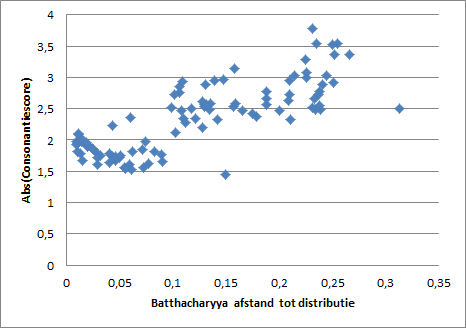
\includegraphics[width=0.75\textwidth]{5_Experimenten_Resultaten/exp11_res}
  \caption{Resultaten van het experiment uitgevoerd in deel \ref{experiment:11}. Absolute waarde van de consonantiescore uitgezet t.o.v. de afstand tot de gemiddelde notendistributie in het Essencorpus.}
  \label{figuur:exp11}
\end{figure}

De resultaten van dit experiment staan weergegeven in figuur \ref{figuur:exp11}. op de y-as staat weer de absolute waarde van de consonantiescore, op de x-as de Bhattacharyya afstand van de notendistributie van het huidige stuk tot de gemiddelde distributie van het Essencorpus. Er is een duidelijk verband merkbaar tussen deze twee waarden. Een stijging van de Bhattacharyya afstand zorgt gemiddeld gezien voor een stijging voor de absolute waarde van de consonantiescore (en dus een verlaging van de probabiliteit van het muziekstukje volgens het RPK-model).

\subsection{Afhankelijkheid score RPK-Model en combinatie metrieken uit experimenten \ref{experiment:10} en \ref{experiment:11}}
\label{experiment:12}
\subsubsection{Beschrijving experiment}
In experimenten \ref{experiment:10} en \ref{experiment:11} werd al duidelijk dat er wel degelijk een verband merkbaar is tussen de consonantiescore en de twee daar besproken metrieken. Het voordeel van deze metrieken was is ze computationeel minder veel minder zwaar zijn dan de berekening van de consonantiescore zelf. De afhankelijkheid was echter telkens niet voldoende om echt als een goede voorspeller beschouwd te worden. Het doel van dit experiment is om te kijken of een combinatie van deze twee metrieken (die beide toch een zeker afhankelijkheid vertonen) misschien tot betere resultaten kan leiden.

In dit experiment wordt voor 100 muziekstukken uit het Essencorpus eerst de consonantiescore bereken. Vervolgens wordt ook het product van de afstand van zijn notendistributie ten opzichte van die van het Essencorpus en de gemiddelde afstand tussen opeenvolgende noten in het muziekstuk berekend.

\subsubsection{Resultaten}
\begin{figure}[!ht]
  \centering
  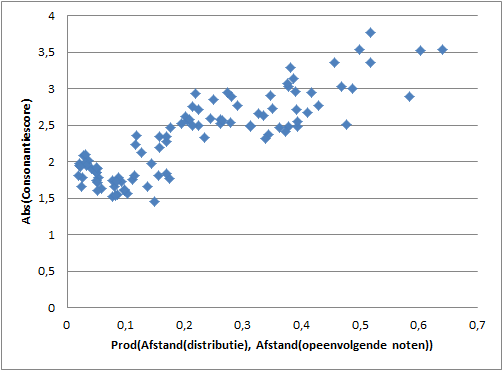
\includegraphics[width=0.75\textwidth]{5_Experimenten_Resultaten/exp12_res}
  \caption{Resultaten van het experiment uitgevoerd in deel \ref{experiment:12}. Absolute waarde van de consonantiescore uitgezet t.o.v. het product van de afstand tot de gemiddelde notendistributie in het Essencorpus en de gemiddelde afstand tussen opeenvolgende noten in het muziekstuk.}
  \label{figuur:exp12}
\end{figure}

De resultaten van dit experiment zijn zichtbaar op figuur \ref{figuur:exp12}. Op de y-as wordt de absolute waarde van de consonantiescore weergegeven. Op de x-as de waarde van het product van de twee afstandsmetrieken die besproken werden. Er is een duidelijk verband merkbaar waarbij een hogere waarde van het product gemiddeld gezien ook leidt tot een hogere absolute waarde van de consonantiescore (en dus een lagere probabiliteit van het muziekstuk).

\section{Experimenten over de werking van de algoritmes voor het combineren van transformaties}
\subsection{Transformaties combineren: 1 transformatie, meerdere iteraties}
\label{experiment:1}
\subsubsection{Beschrijving experiment}
Dit experiment heeft betrekking tot het algoritme dat besproken werd in onderdeel \ref{ETT:algo1}. Dit experiment gaat nagaan wat de invloed is van het aantal iteraties van het aantal iteraties van dit algoritme op de consonantiescore van het totale muziekstuk. Er wordt in dit algoritme slechts gebruik gemaakt van een transformatie. Deze gebruikte transformatie wordt weergegeven in tabel \ref{tabel:exp1}.

\begin{table}
  \centering
  \begin{tabular}{c | c c c c c c c c }
    Diff (mod 8) & 0 & 1 & 2 & 3 & 4 & 5 & 6 & 7 \\
    \hline
    \hline
    Verhoging & 5 & -4 & 1 & -3 & 1 & 1 & 2 & 3 \\
  \end{tabular}
  \caption{Transformatie gebruikt in het experiment van onderdeel \ref{experiment:1}.}
  \label{tabel:exp1}
\end{table}

Deze test wordt uitgevoerd op 100 muziekstukken uit het Essencorpus. De gemiddelde probabiliteit van de originele stukken wordt berekend alsook de gemiddelde probabiliteit van het muziekstuk dat optimaal is volgens het RPK-model in de toonaard van de 100 stukken. Nu kan er gekeken worden naar hoe snel de consonantiescore zich gaat verplaatsten van die van het originele naar die van de theoretisch best mogelijke volgens het model afhankelijk van het aantal iteraties dat het algoritme wordt uitgevoerd.

\subsubsection{Resultaten}
\begin{figure}[!ht]
  \centering
  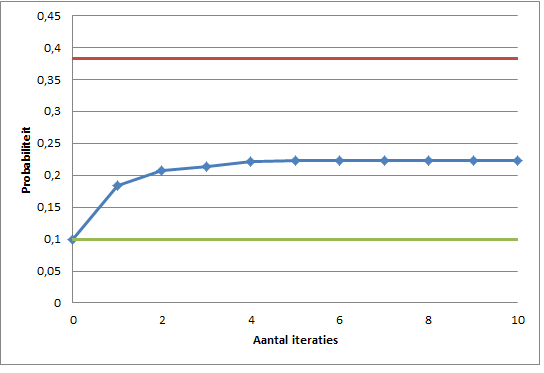
\includegraphics[width=0.75\textwidth]{5_Experimenten_Resultaten/exp1_res}
  \caption{Resultaten van het experiment uitgevoerd in deel \ref{experiment:1}. De groene lijn staat voor de gemiddelde probabiliteit van een noot in de originele melodie, de rode lijn voor de gemiddelde probabiliteit van de theoritisch beste melodielijn in de toonaarden waarop getest werd en de blauwe lijn geeft de gemiddelde probabiliteit van een noot weer na uitvoer van het algoritme na een verschillend aantal iteraties.}
  \label{figuur:exp1}
\end{figure}

In figuur \ref{figuur:exp1} worden de restultaten weergegeven van dit experiment. De groene lijn op de figuur geeft de gemiddelde probabiliteit weer van alle melodie\"en waarop getest werd. De rode lijn geeft voor al deze melodie\"en de gemiddelde waarde mee voor het theoretisch beste muziekstuk dat volgens het RPK-model gemaakt kan worden in deze toonaard. Tot slot geeft de blauwe lijn de gemiddelde probabiliteit weer van een noot in de getransformeerde melodie, na toepassing van 1 tot 10 iteraties van de transformatie.\\
Er valt duidelijk op dat de eerste paar iteraties nog een redelijke verhoging van de probabiliteit teweeg brengt, maar dat na een vijftal iteraties gemiddeld gezien een soort van maximum bereikt is dat met deze transformatie kan bekomen worden. De reden dat deze waarde nog zo ver onder het theoretische maximum ligt, heeft er vooral mee te maken dat er maar 1 mogelijke transformatie is dat het algoritme mag gebruiken, hierdoor zijn er nog steeds maar een zeer beperkt aantal mogelijkheiden om een bepaalde noot te transformeren, en kunnen bijgevolg nog steeds de meeste noten niet bereikt worden vanuit eender welke noot.

\subsection{Transformaties combineren: meerdere transformaties, 1 iteratie}
\label{experiment:2}
\subsubsection{Beschrijving experiment}
Dit experiment heeft betrekking tot het algoritme dat besproken werd in onderdeel \ref{ETT:algo1}. Het experiment gaat nagaan wat de invloed is van het aantal verschillende toegelaten transformaties op de consonantiescore van het totale muziekstuk. Zo zijn de vijf transformaties die gebruikt zullen worden weergegeven in tabel \ref{tabel:exp2}. Er wordt nu telkens slechts een iteratie van het algoritme uitgevoerd.\\

\begin{table}
  \centering
  \begin{tabular}{c | c c c c c c c c }
    Diff (mod 8) & 0 & 1 & 2 & 3 & 4 & 5 & 6 & 7 \\
    \hline
    \hline
    Verhoging transformatie 1 & 5 & -4 & 1 & -3 & 1 & 1 & 2 & 3 \\
    \hline
    Verhoging transformatie 2 & 1 & 3 & 4 & -5 & -1 & 6 & 5 & -1 \\
    \hline
    Verhoging transformatie 3 & 1 & 4 & 5 & -3 & 2 & -1 & 1 & 0 \\
    \hline
    Verhoging transformatie 4 & 4 & 6 & -2 & 4 & 2 & 6 & -4 & 2 \\
    \hline
    Verhoging transformatie 5 & -3 & -2 & 3 & -1 & 4 & -3 & 2 & -4 \\
  \end{tabular}
  \caption{Transformaties gebruikt in het experiment van onderdeel \ref{experiment:2}.}
  \label{tabel:exp2}
\end{table}

Deze test wordt uitgevoerd op 50 muziekstukken uit het Essencorpus. De gemiddelde probabiliteit van de originele stukken wordt berekend alsook de gemiddelde probabiliteit van het muziekstuk dat optimaal is volgens het RPK-model in de toonaard van de 50 stukken. Nu kan er weer gekeken worden naar hoe snel de consonantiescore zich gaat verplaatsten van die van het originele naar die van de theoretisch best mogelijke volgens het model afhankelijk van het aantal transformaties dat aan het algoritme ter beschikking wordt gesteld. Het experiment wordt eerst uitgevoerd met slechts een mogelijke transformatie. Dit zal dan transformatie 1 uit de tabel zijn. Daarna wordt het experiment uitgevoerd met 2 mogelijke transformaties. Dit zullen dan de eerste twee transformaties uit de tabel zijn enz..

\subsubsection{Resultaten}
\begin{figure}[!ht]
  \centering
  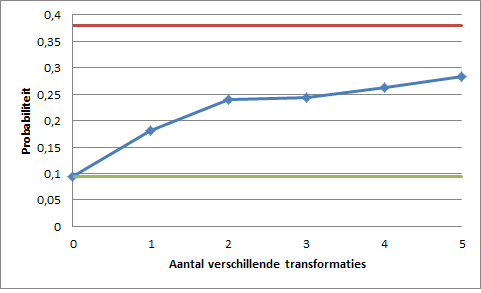
\includegraphics[width=0.75\textwidth]{5_Experimenten_Resultaten/exp2_res}
  \caption{Resultaten van het experiment uitgevoerd in deel \ref{experiment:2}. De groene lijn staat voor de gemiddelde probabiliteit van een noot in de originele melodie, de rode lijn voor de gemiddelde probabiliteit van de theoritisch beste melodielijn in de toonaarden waarop getest werd en de blauwe lijn geeft de gemiddelde probabiliteit van een noot weer na uitvoer van het algoritme afhankelijk van het aantal transformaties dat ter beschikking gesteld was aan het algoritme.}
  \label{figuur:exp2}
\end{figure}

In figuur \ref{figuur:exp2} worden de restultaten weergegeven van dit experiment. Het is duidelijk dat een  hoger aantal transformaties ook telkens een betere score teruggeeft. Als we de resultaten van dit experiment vergelijken met dat uit onderdeel \ref{experiment:1}, dan merken we op dat het aantal transformaties een grotere impact heeft op de probabiliteit dan het aantal iteraties. De grootste reden hiervoor is dat een extra transformaties er voor kan zorgen dat er voor elke een noot in het muziekstuk een extra mogelijke noot is waarnaar hij getransformeerd kan worden. Dit zorgt voor enorm veel extra mogelijkheden waardoor er hogere probabiliteiten kunnen bekomen worden dan in het geval waarbij het aantal iteraties verhoogd wordt in plaats van het aantal mogelijke transformaties.  


\subsection{Transformaties combineren: minimum transformatie lengte}
\label{experiment:3}
\subsubsection{Beschrijving experiment}
Dit experiment heeft betrekking tot het algoritme dat besproken werd in onderdeel \ref{ETT:algo2}. Het experiment gaat nagaan wat de invloed is van de minimum transformatielengte op de consonantiescore van het totale muziekstuk. Er wordt in dit experiment telkens gebruik gemaakt van 2 transformaties die beschreven zijn in tabel \ref{tabel:exp3}. Er wordt telkens slechts een iteratie van het algoritme uitgevoerd.\\

\begin{table}
  \centering
  \begin{tabular}{c | c c c c c c c c }
    Diff (mod 8) & 0 & 1 & 2 & 3 & 4 & 5 & 6 & 7 \\
    \hline
    \hline
    Verhoging transformatie 1 & 5 & -4 & 1 & -3 & 1 & 1 & 2 & 3 \\
    \hline
    Verhoging transformatie 2 & 1 & 3 & 4 & -5 & -1 & 6 & 5 & -1 \\
  \end{tabular}
  \caption{Transformaties gebruikt in het experiment van onderdeel \ref{experiment:3}.}
  \label{tabel:exp3}
\end{table}

Dit experiment wordt uitgevoerd op 50 muziekstukken uit het Essencorpus en dit voor alle waarden van de minimum transformatie lengte tussen 1 en 10. Voor elk van deze 10 gevallen wordt de gemiddelde probabiliteit van het getransformeerde muziekstuk berekend.

\subsubsection{Resultaten}
\begin{figure}[!ht]
  \centering
  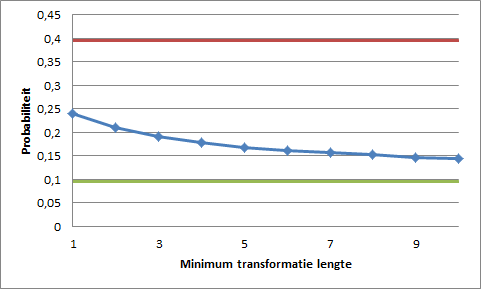
\includegraphics[width=0.75\textwidth]{5_Experimenten_Resultaten/exp3_res}
  \caption{Resultaten van het experiment uitgevoerd in deel \ref{experiment:3}. De groene lijn staat voor de gemiddelde probabiliteit van een noot in de originele melodie, de rode lijn voor de gemiddelde probabiliteit van de theoritisch beste melodielijn in de toonaarden waarop getest werd en de blauwe lijn geeft de gemiddelde probabiliteit van een noot weer na uitvoer van het algoritme afhankelijk van de minimum transformatie lengte.}
  \label{figuur:exp3}
\end{figure}

Figuur \ref{figuur:exp3} geeft de resultaten weer van het experiment. Het is duidelijk dat een hogere minimum transformatie lengte leidt tot een kleinere verbetering van de consonantiescore, wat te verwachten was. De grafiek is ook monotoon dalen voor stijgende waarde van de minimum transformatie lengte. Dit moet ook zo zijn aangezien alle transformaties die geldig zijn voor een zekere transformatie lengte ook altijd geldig zijn voor alle kortere transformatie lengtes.

\subsection{Transformaties combineren: Gelijkheid algoritmen voor transformatie lengte 1}
\label{experiment:4}
\subsubsection{Beschrijving experiment}
Dit experiment is opgezet als extra test om het geloof in de juiste werking van de algoritmes beschreven in \ref{ETT:algo1} en \ref{ETT:algo2} te versterken. Aangezien de implementaties van deze twee algoritmen toch op een aantal vlakken (vooral de voorstelling van de paden) verschillen van elkaar, is het interessant om voor een minimum transformatie lengte van 1 eens te kijken of de twee algoritmes hetzelfde resultaat geven. Dit zou normaal gezien altijd het geval moeten zijn aangezien de twee algoritmes hetzelfde doel en dezelfde middelen hebben in het geval van een minimum transformatie lengte van 1. De transformatie waarvan gebruik gaat worden gemaakt staat beschreven in tabel \ref{tabel:exp4}.

\begin{table}
  \centering
  \begin{tabular}{c | c c c c c c c c }
    Diff (mod 8) & 0 & 1 & 2 & 3 & 4 & 5 & 6 & 7 \\
    \hline
    \hline
    Verhoging & 5 & -4 & 1 & -3 & 1 & 1 & 2 & 3 \\
  \end{tabular}
  \caption{Transformatie gebruikt in het experiment van onderdeel \ref{experiment:4}.}
  \label{tabel:exp4}
\end{table}

Voor deze transformatie gaat het experiment zoals het beschreven staat in onderdel \ref{experiment:1} herhaald worden maar dan ook voor het tweede algoritme. Dus voor een aantal iteraties van 1 tot en met 10 van het algoritme gaan de probabiliteiten die beide algoritmes opleveren voor dezelfde transformatie op dezelfde 100 testgevallen uit het Essencorpus vergeleken worden.

\subsubsection{Resultaten}
\begin{table}
  \centering
  \begin{tabular}{c | c | c }    
    \# iteraties & Algoritme 1 & Algoritme 2 \\
    \hline
    1 & -1.69 & -1.69\\
    2 & -1.57 & -1.57\\
    3 & -1.54 & -1.54\\
    4 & -1.51 & -1.51\\
    5 & -1.50 & -1.50\\
    6 & -1.50 & -1.50\\
    7 & -1.50 & -1.50\\
    8 & -1.50 & -1.50\\
    9 & -1.50 & -1.50\\
    10 & -1.50 & -1.50\\
  \end{tabular}
  \caption{Resulaten van experiment \ref{experiment:4}. Gemiddelde consonantiescores voor de twee algoritmen (logaritme van de probabiliteit) na een gegeven aantal iteraties. Algoritme 1 staat beschreven in \ref{ETT:algo1}, algoritme 2 is hetgene dat beschreven staat in \ref{ETT:algo2}.}
  \label{tabel:res4}
\end{table}

In tabel \ref{tabel:res4} staan de resultaten van dit experiment weergegeven. Beide algoritmen leveren dezelfde gemiddelde consonantiescore (logaritme van de gemiddelde probabiliteit) voor een muziekstukje na eenzelfde aantal iteraties gebruik makende van dezelfde transformatie. Dit versterkt de stelling dat de twee algoritmes wel degelijk werken zoals gewenst.

\section{Experimenten over de tijdscomplexiteit van de algoritmes voor het combineren van transformaties}
\subsection{Tijdsafhankelijkheid algoritme \ref{ETT:algo2} van het aantal noten in de melodielijn}
\label{experiment:7}
\subsubsection{Beschrijving experiment}
Van het algoritme beschreven in onderdeel \ref{ETT:algo2} werd reeds beargumenteerd dat de uitvoertijd lineair afhankelijk is van het aantal noten van de originele melodielijn. De bedoeling is nu om experimenteel na te gaan of dit wel klopt. Om dit te testen wordt gebruik gemaakt van een transformatie die beschreven staat in tabel \ref{tabel:exp7}.

\begin{table}
  \centering
  \begin{tabular}{c | c c c c c c c c }
    Diff (mod 8) & 0 & 1 & 2 & 3 & 4 & 5 & 6 & 7 \\
    \hline
    \hline
    Verhoging & 1 & 1 & 2 & 3 & 5 & -4 & 1 & -3 \\
  \end{tabular}
  \caption{Transformatie gebruikt in het experiment van onderdeel \ref{experiment:7}.}
  \label{tabel:exp7}
\end{table}

Voor 20 verschillende lengtes van melodielijnen (10 tot en met 200 met stapgrootte 10) wordt nu de uitvoertijd gemeten. Hierna kan de uitvoertijd van het algoritme uitgezet worden ten opzicht van de invoergrootte en zou er een lineair verband zichtbaar moeten zijn.

\subsubsection{Resultaten}
\begin{figure}[!ht]
  \centering
  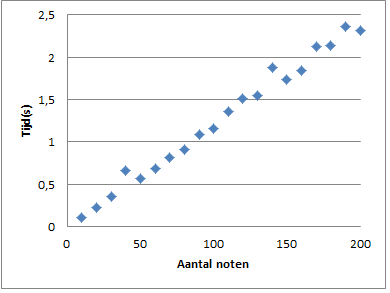
\includegraphics[width=0.75\textwidth]{5_Experimenten_Resultaten/exp7_res}
  \caption{Resultaten van het experiment uitgevoerd in deel \ref{experiment:7}. Tijdsduur van het algoritme in seconden t.o.v. het aantal noten in de originele melodie.}
  \label{figuur:exp7}
\end{figure}

In figuur \ref{figuur:exp7} worden de resultaten van dit experiment weergegeven in een scatter plot. Er is een duidelijk lineair verband zichtbaar tussen de grootte van de melodielijn en de uitvoertijd. Dit komt overeen met de afhankelijkheid die beredeneerd werd in hoofdstuk \ref{ETT:algo2}.

\subsection{Tijdsafhankelijkheid algoritme \ref{ETT:algo2} van aantal toegelaten transformaties}
\label{experiment:8}
\subsubsection{Beschrijving experiment}
Dit experiment heeft betrekking op het algoritme beschreven in hoofdstuk \ref{ETT:algo2}. Er werd gesteld dat de uitvoertijd van dit algoritme evenredig is met het kwadraat van het aantal toegelaten transformaties. De bedoeling van dit experiment is om na te gaan of deze beredenering kan kloppen door voor verschillende aantallen transformaties te berekenen hoelang het algoritme nodig heeft om eenzelfde invoer te verwerken. De tien transformaties die gebruikt worden in dit experiment staan beschreven in tabel \ref{tabel:exp8}. Het maakt voor de snelheid va uitvoer van het algoritme geen verschil welke transformaties er meegegeven worden (10 dezelfde transformaties duren even lang om te verwerken dan 10 verschillende), maar voor de volledigheid zijn de transformaties hier toch weergegeven aangezien deze gebruikt werden tijdens het experiment.

\begin{table}
  \centering
  \begin{tabular}{c | c c c c c c c c }
    Diff (mod 8) & 0 & 1 & 2 & 3 & 4 & 5 & 6 & 7 \\
    \hline
    \hline
    Verhoging transformatie 1 & 5 & -4 & 1 & -3 & 1 & 1 & 2 & 3 \\
    \hline
    Verhoging transformatie 2 & 1 & 3 & 4 & -5 & -1 & 6 & 5 & -1 \\
    \hline
    Verhoging transformatie 3 & 1 & 4 & 5 & -3 & 2 & -1 & 1 & 0 \\
    \hline
    Verhoging transformatie 4 & 4 & 6 & -2 & 4 & 2 & 6 & -4 & 2 \\
    \hline
    Verhoging transformatie 5 & -3 & -2 & 3 & -1 & 4 & -3 & 2 & -4 \\
    \hline
    Verhoging transformatie 6 & 1 & 1 & 2 & 3 & 5 & -4 & 1 & -3 \\
    \hline
    Verhoging transformatie 7 & -1 & 6 & 5 & -1 & 2 & 1 & 3 & 4 \\
    \hline
    Verhoging transformatie 8 & 2 & -1 & 1 & 0 & 3 & 1 & 4 & 5 \\
    \hline
    Verhoging transformatie 9 & 2 & 6 & -4 & 2 & 4 & 6 & -2 & 4 \\
    \hline
    Verhoging transformatie 10 & 4 & -3 & 2 & -4 & -3 & -2 & 3 & -1 \\
  \end{tabular}
  \caption{Transformaties gebruikt in het experiment van onderdeel \ref{experiment:8}.}
  \label{tabel:exp8}
\end{table}

Voor eenzelfde melodielijn wordt 10 keer het algoritme uitgevoerd. De eerste keer heeft het algoritme enkel `transformatie' 1 ter beschikking. De tweede keer heeft het algoritme zowel `transformatie 1' als `transformatie 2' ter beschikking, enz..

\subsubsection{Resultaten}
\begin{figure}[!ht]
  \centering
  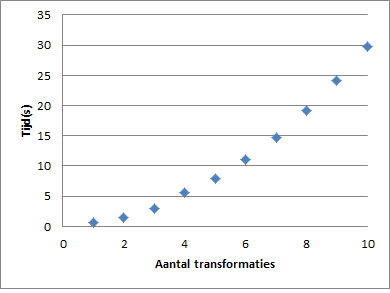
\includegraphics[width=0.75\textwidth]{5_Experimenten_Resultaten/exp8_res}
  \caption{Resultaten van het experiment uitgevoerd in deel \ref{experiment:8}. Tijdsduur van het algoritme in seconden t.o.v. het aantal transformaties dat het algoritme ter beschikking heeft.}
  \label{figuur:exp8}
\end{figure}

De resultaten van dit experiment staan weergegeven in een scatter plot in figuur \ref{figuur:exp8}. Op deze figuur lijkt een kwadratische afhankelijkheid tussen het aantal beschikbaren transformaties en de uitvoertijd van het algoritme zichtbaar. Dit komt overeen met de beredeneerde afhankelijkheid van in hoofdstuk \ref{ETT:algo2}.

\subsection{Tijdsafhankelijkheid algoritme \ref{ETT:algo2} van minimum transformatie lengte}
\label{experiment:9}
\subsubsection{Beschrijving experiment}
Van het algoritme beschreven in hoofdstuk \ref{ETT:algo2} werd reeds beredeneerd dat de uitvoertijd van het algoritme afhankelijk is van $ML \times (AN-ML)$. Met ML, de minimum transformatie lengte en AN het aantal noten in de originele melodie. De bedoeling van dit experiment is om na te gaan of deze beredeneerde afhankelijkheid ook zichtbaar is in realiteit. Het algoritme kreeg tijdens dit experiment telkens twee transformaties ter beschikking, deze staan beschreven in tabel \ref{tabel:exp9}.

\begin{table}
  \centering
  \begin{tabular}{c | c c c c c c c c }
    Diff (mod 8) & 0 & 1 & 2 & 3 & 4 & 5 & 6 & 7 \\
    \hline
    \hline
    Verhoging transformatie 1 & 5 & -4 & 1 & -3 & 1 & 1 & 2 & 3 \\
    \hline
    Verhoging transformatie 2 & 1 & 1 & 2 & 3 & 5 & -4 & 1 & -3 \\
  \end{tabular}
  \caption{Transformaties gebruikt in het experiment van onderdeel \ref{experiment:9}.}
  \label{tabel:exp9}
\end{table}

In dit experiment wordt telkens eenzelfde melodielijn met een lengte van 30 noten (dus AN=30) meegegeven aan het algoritme. En nu wordt voor 30 verschillende waarden van de minimum transformatie lengte (ML van 1 tot en met 30), het algoritme uitgevoerd.

\subsubsection{Resultaten}
\begin{figure}[!ht]
  \centering
  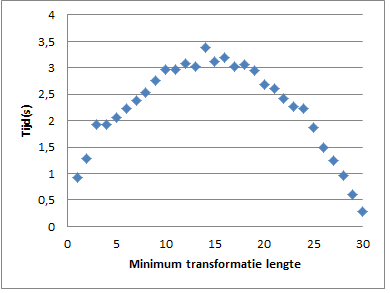
\includegraphics[width=0.75\textwidth]{5_Experimenten_Resultaten/exp9_res}
  \caption{Resultaten van het experiment uitgevoerd in deel \ref{experiment:9}. Tijdsduur van het algoritme in seconden t.o.v. de opgelegde minimum transformatie lengte.}
  \label{figuur:exp9}
\end{figure}

De resultaten van dit experiment zijn zichtbaar op de scatter plot van figuur \ref{figuur:exp9}. Dit experiment lijkt de stelling dat de uitvoertijd afhankelijk is van $ML \times (AN-ML)$ te staven.



%%% Local Variables: 
%%% mode: latex
%%% TeX-master: "masterproef"
%%% End: 

\chapter{Besluit}
\label{hoofdstuk:B}


%%% Local Variables: 
%%% mode: latex
%%% TeX-master: "masterproef"
%%% End: 


% Indien er bijlagen zijn:
\appendixpage*          % indien gewenst
\appendix
\chapter{Broncode}
\label{app:broncode}

\section{Neuraal netwerk trainer}
\label{Broncode:ANN}
\lstinputlisting[language = Java, frame=single]{Appendix_0_Broncode/NeuralNetworkTrainer.java}

\section{RPK-model}
\label{Broncode:RPK}
\lstinputlisting[language = Python, frame=single]{Appendix_0_Broncode/RPK.py}

\section{Beste sequentie}
\label{Broncode:algo1}
\lstinputlisting[language = Python, frame=single]{Appendix_0_Broncode/BestSequenceCleaned.py}

\section{Beste sequentie met minimum transformatie lengte}
\label{Broncode:algo2}
\lstinputlisting[language = Python, frame=single]{Appendix_0_Broncode/BestCoordinatedSequenceCleaned.py}

%%% Local Variables: 
%%% mode: latex
%%% TeX-master: "masterproef"
%%% End: 

\chapter{IEEE\_Paper}
\label{app:paper}
In de bijlagen vindt men de data terug die nuttig kunnen zijn voor de
lezer, maar die niet essentieel zijn om het betoog in de normale tekst te
kunnen volgen. Voorbeelden hiervan zijn bronbestanden,
configuratie-informatie, langdradige wiskundige afleidingen, enz.

In een bijlage kunnen natuurlijk ook verdere onderverdelingen voorkomen,
evenals figuren en referenties\cite{h2g2}.

%%% Local Variables: 
%%% mode: latex
%%% TeX-master: "masterproef"
%%% End: 

\chapter{Poster}
\label{app:poster}

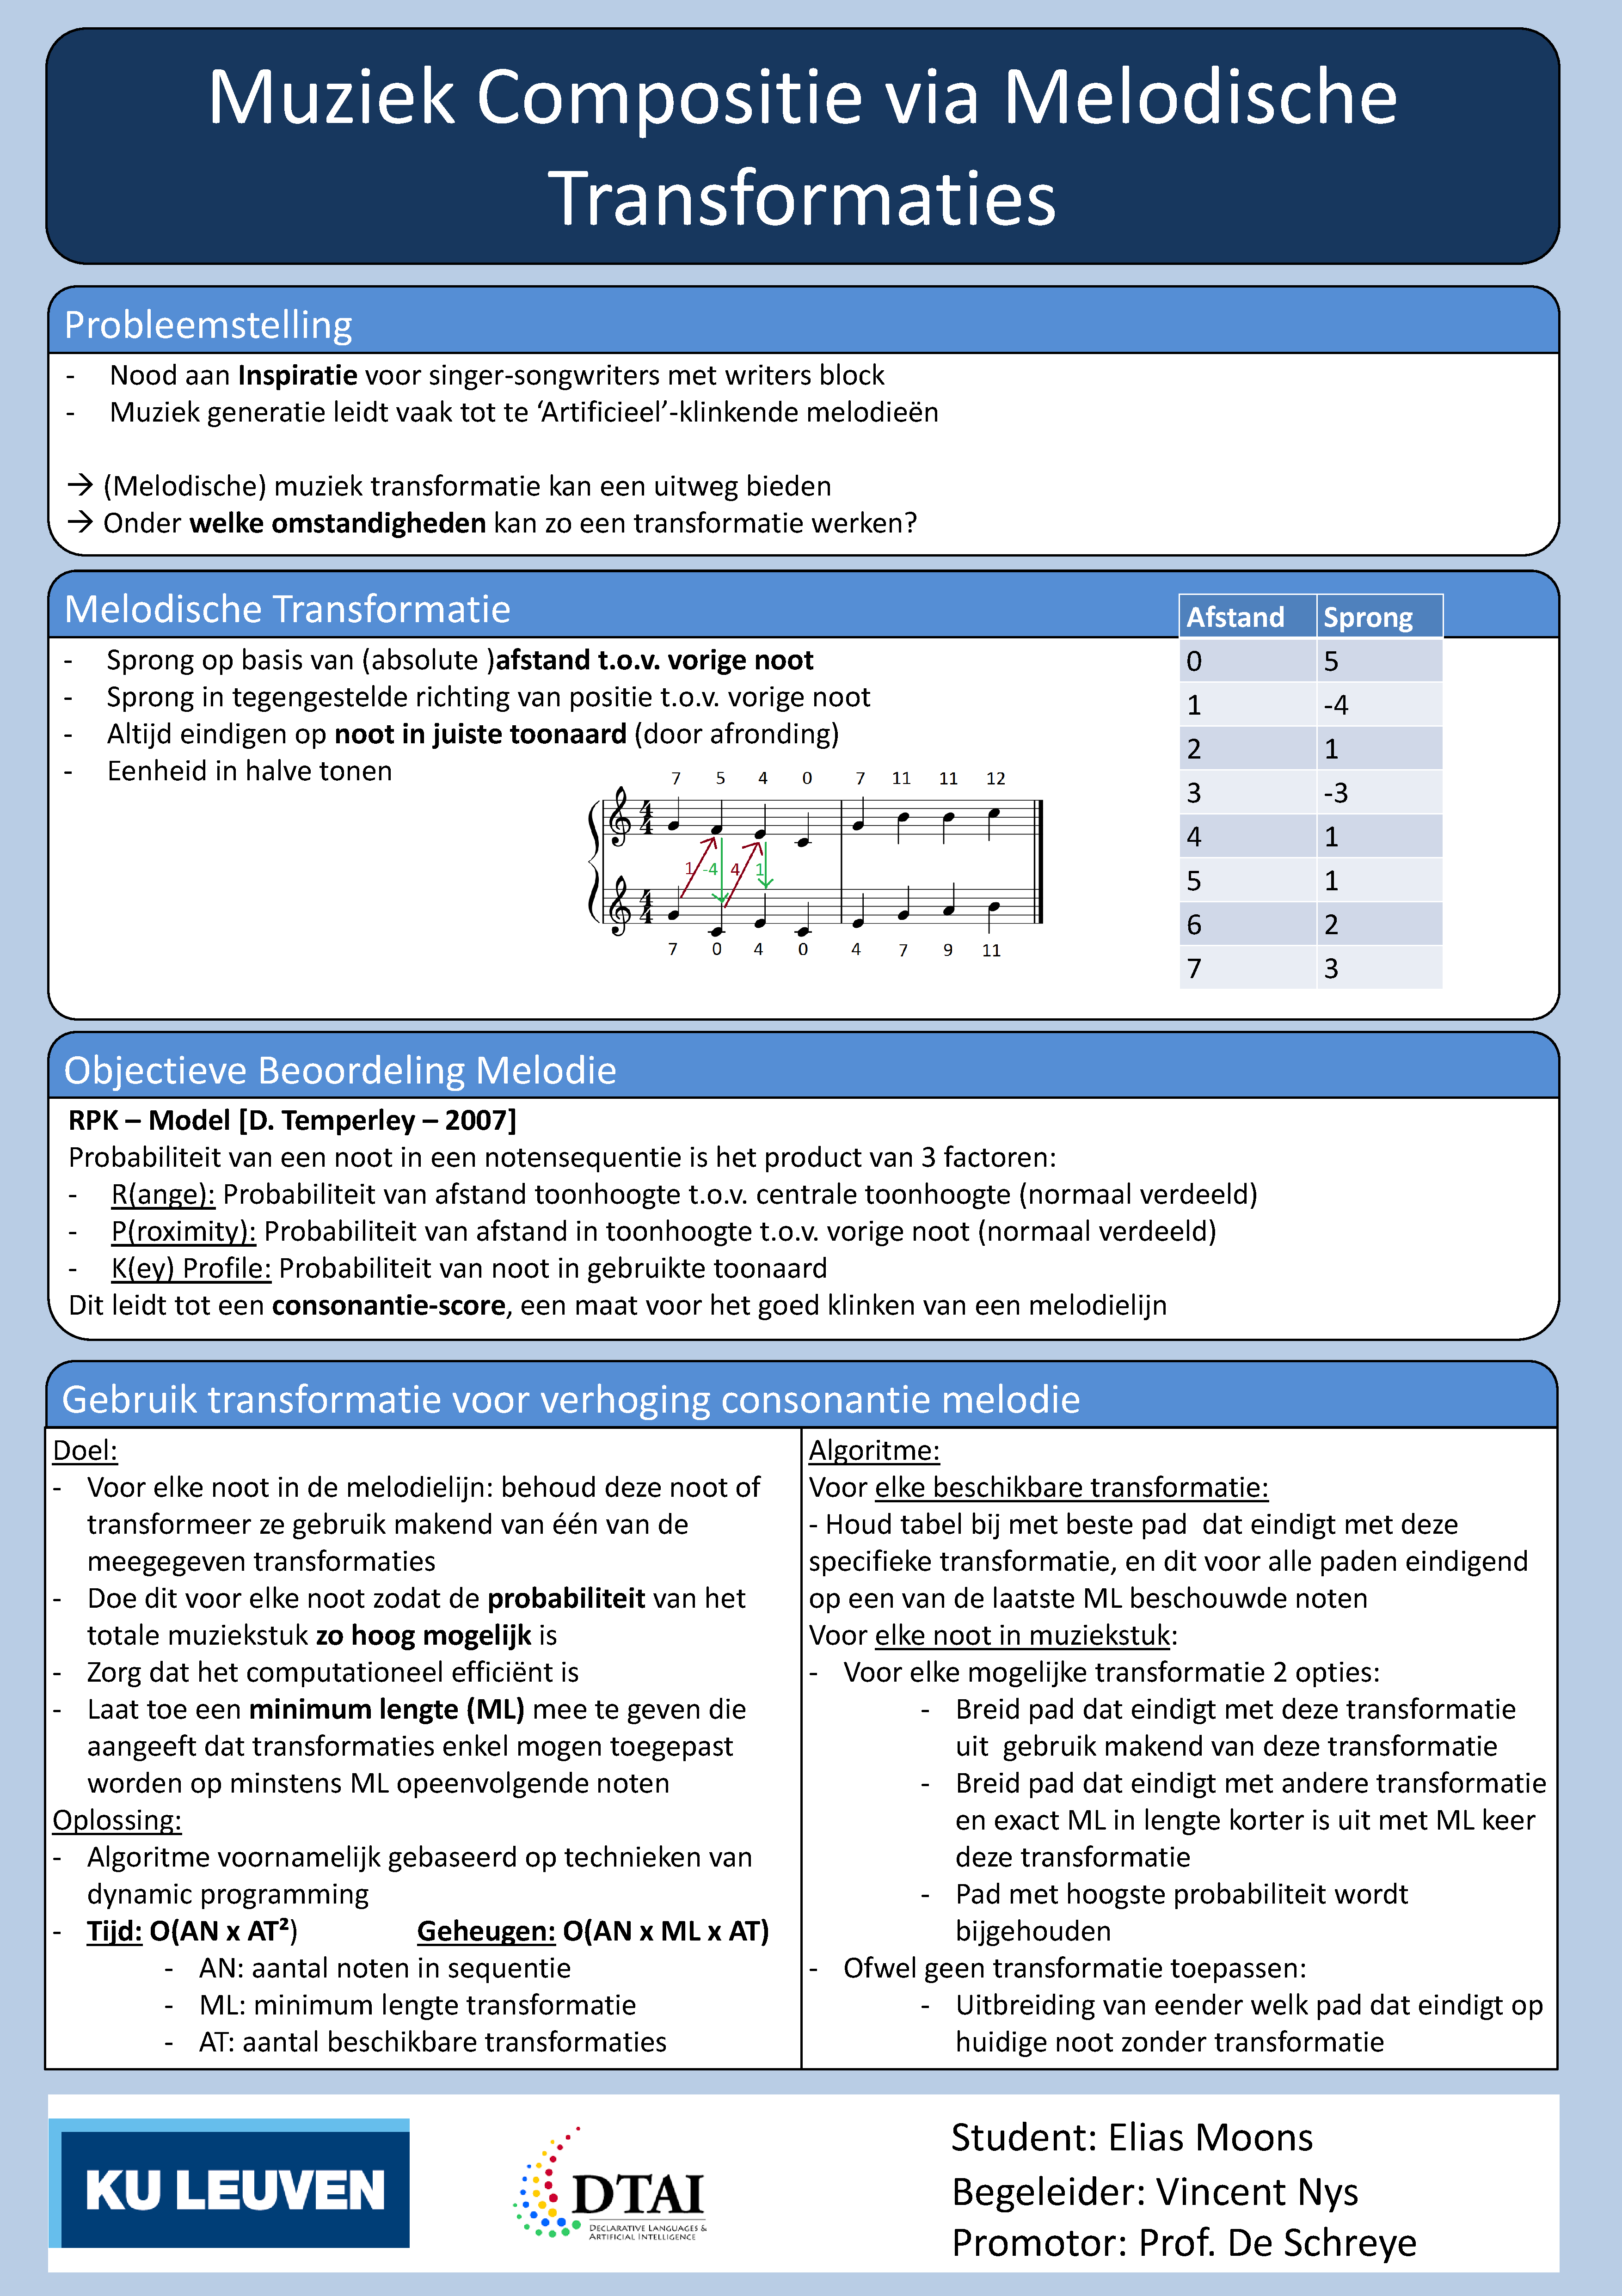
\includepdf[pages={1}]{Appendix_2_Poster/Poster_EliasMoons.pdf}

%%% Local Variables: 
%%% mode: latex
%%% TeX-master: "masterproef"
%%% End: 



\backmatter
% Na de bijlagen plaatst men nog de bibliografie.
% Je kan de  standaard "abbrv" bibliografiestijl vervangen door een andere.
\bibliographystyle{abbrv}
\bibliography{referenties}

\end{document}

%%% Local Variables: 
%%% mode: latex
%%% TeX-master: t
%%% End: 
